%------------------------------------------------------------------------------
% Template file for the submission of papers to IUCr journals in LaTeX2e
% using the iucr document class
% Copyright 1999-2013 International Union of Crystallography
% Version 1.6 (28 March 2013)
%------------------------------------------------------------------------------
%
%
% \documentclass{iucr}
\documentclass[preprint]{iucr}              % DO NOT DELETE THIS LINE
\usepackage{bm}
\usepackage{mathtools}
\usepackage{amssymb}
\usepackage{amsmath}
\usepackage{siunitx}
\usepackage[hyphens,spaces,obeyspaces]{url}
\usepackage{color}
\usepackage{textgreek}
\usepackage[normalem]{ulem}
\usepackage{makecell}
\usepackage{cancel}
\usepackage{empheq}
\usepackage[usenames,dvipsnames]{xcolor}
\usepackage{enumitem}

\definecolor{darkblue}{rgb}{0.0, 0.0, 0.55}
\definecolor{cyan(process)}{rgb}{0.0, 0.72, 0.92}

\newcommand{\todo}[1]{{\color{red}[TODO: "#1'']}}
\newcommand{\inblue}[1]{{\color{blue}#1}}
\newcommand{\cyan}[1]{{\color{cyan(process)}#1}}
\newcommand{\inred}[1]{{\color{red}#1}}
\newcommand{\ingreen}[1]{{\color{green}#1}}



\makeatletter
\@ifclasswith{iucr}{preprint}{
\newcommand{\whencolumns}[2]{#1}
}{
\newcommand{\whencolumns}[2]{#2}
}
\makeatother

     %-------------------------------------------------------------------------
     % Infobrmation about journal to which submitted
     %-------------------------------------------------------------------------
     \journalcode{X}              % Indicate the journal to which submitted
                                  %   A - Acta Crystallographica Section A
                                  %   B - Acta Crystallographica Section B
                                  %   C - Acta Crystallographica Section C
                                  %   D - Acta Crystallographica Section D
                                  %   E - Acta Crystallographica Section E
                                  %   F - Acta Crystallographica Section F
                                  %   J - Journal of Applied Crystallography
                                  %   M - IUCrJ
                                  %   S - Journal of Synchrotron Radiation

\begin{document}  % DO NOT DELETE THIS LINE

\title{Semianalytical implementation of Laue crystals in simulations of wavefront propagation}


\author{Manuel}{Sanchez del Rio}
\author{Jean-Pierre}{Guigay}


\aff{European Synchrotron Radiation Facility, {71 Avenue des Martyrs} 38000 Grenoble France}

\maketitle   % DO NOT DELETE THIS LINE

\begin{synopsis}
Curved Laue crystals are implemented in the wavefront-propagation code WOFRY using a semi-analytical crystal propagator derived from the dynamical theory of diffraction; the implementation is benchmarked against published results and applied to the design of bent-crystal monochromators.
\end{synopsis}

\begin{abstract}

We present here the implementation of curved Laue crystals in a wave optics propagation simulation tool. We calculate the crystal propagator using equations of the dynamical theory of diffraction recently developed \cite{GuigayFerrero2016} to study the focusing of these crystals. We present the implementation, we benchmark it against some published results and discuss some practical cases where these calculations can be useful.

\end{abstract}


%%%%%%%%%%%%%%%%%%%%%%%%%%%%%%%%%%%%%%%%%%%%%%%%%%%%
%
%%%%%%%%%%%%%%%%%%%%%%%%%%%%%%%%%%%%%%%%%%%%%%%%%%%%
\section{Introduction}
\label{sec:Intro}

Simulations of beamline optics can be done in different degrees of approximation, starting from analytical formulas, performing ray-tracing, and also wavefront propagation \cite{hyerarchical}. Different packages for such simulations are available in the OASYS suite \cite{codeOASYS}. For incoherent photon beams, the ray-tracing technique is suitable for most purposes.
If the X-ray beam is highly coherent, a pure wave-optics simulation is usually sufficient.
Hard X-rays produced by new or upgraded synchrotron storage rings have a coherent fraction typically of a few percent. Accurate simulations for these beams require using hybrid methods \cite{hybrid} or more sophisticated partial coherence algorithms such as Monte Carlo sampling \cite{Chubar2011b} and Coherent Mode Decomposition \cite{glassEPL}. 

We consider here crystals in transmission geometry (Laue) and we want to simulate their effect in a beamline or other optical system. 
Crystals in transmission or Laue geometry are often employed in beamlines operating at high photon energies, because the small Bragg angles and narrow Darwin width make difficult the use of the common reflection geometry (Bragg).
Moreover, the crystal curvature in Laue crystal configuration can be used to focus (or collimate) the beam in the meridional \cite{Suortti1988,SuorttiShulze} or sagittal \cite{Zhong2001} directions, or just to enlarge the energy bandwidth and improve the luminosity. 
The crystal bandwidth was optimized and aberrations reduced thanks to the high collimation and small source size of synchrotron beams. 
We discuss the implementation of curved Laue crystals in a wavefront propagation framework. 

We remind that the applicability of ``simple models" of focusing predicted by a ``lens equation" for the Laue crystals is limited to very thin crystals \cite{guigaySanchezdelrio2022}.
The dynamical theory [see book \cite{authierbook}] predicts ``new" focal conditions, even for flat Laue crystals.
This was analyzed in \cite{Kohn2000} \inred{??} in the framework of the Takagi-Taupin equations \cite{Takagi1962, Takagi, Taupin, Taupin1967}. The dynamical effects produced by diffraction over the Borrmann triangle produce a wavefront, that is not plane neither spherical, that can evolve (propagate) in a complex manner, creating two focal points [see \cite{Nesterets2008, GuigayFerrero2013, GuigayFerrero2016}].
Moreover, this ``monochromatic" focusing can be combined with ``polychromatic" focusing and other geometrical effects \cite{PengQi, PengQi2021}, thus making particularly complex the simulation of these crystals in optical systems like synchrotron beamlines. It usually requires a wave optics treatment to take into account dynamical effects, because the simple geometrical models or ray propagation have limitations.  

SRW (Synchrotron Radiation Workshop) \cite{codeSRW} is an open‑source physical‑optics (wave‑optics) simulation package.
SRW includes a perfect‑crystal propagator to handle Bragg‑case dynamical diffraction from ideal flat crystals \cite{codeSRWcrystals}.
The method decomposes the incident field by Fourier Transform (FT) into the angular (plane‑wave) domain. Then it applies the standard dynamical‑diffraction theory for plane waves \cite{ZachariasenBook} to each Fourier component. 
Finally it applies the inverse‑FT back to real domain. 
The method \inred{seamlessly} integrates with SRW’s existing drift‑space, aperture, lens and mirror propagators, allowing full‑field simulations of coherent X‑ray beams that pass through Bragg monochromator crystals.
Even though this implementation is limited to the case of flat crystals in reflection (Bragg), the underlying idea of how the crystal acts and modifies the input wavefront is interesting: the crystal ``diffraction profiles" (crystal reflectivity vs angle) are used to calculate the diffraction effect on a generic input wavefront by a model that is equivalent to: 
\begin{enumerate}
    \item express the incident wave as a sum of plane waves (FT, equivalent to propagation to far field),
    \item apply the crystal reflectivity (complex amplitude vs. angle) to each component, and
    \item back-propagate the modified far field to the crystal position (inverse FT).
\end{enumerate}
\todo{Is this approach similar to the one used by Kato, Petrashen, Kohn? Find references.}


WOFRY \cite{WOFRYoptics} is a wavefront propagation tool available in the OASYS suite \cite{OASYS}. 
Several optical elements are implemented, including absorbers (slits and stops), reflectors (mirrors and gratings), and refractors (ideal lenses: defined solely by the focal length; real lenses: including the shape of interfaces and material absorption; compound refractive lenses, and thin objects \cite{Celestre2019}).
In this paper we present the physical model and discuss some results of the new Laue Crystal component in the WOFRY system.

% -----------------------------------------------------------------
% -----------------------------------------------------------------
\section{Summary of wavefront simulations with WOFRY}


We use wavefronts that are defined in a plane perpendicular to the main propagation direction. We define the propagation direction $y$. In a 2D model, the plane perpendicular to the propagation direction has coordinates $(x,z)$ (horizontal and vertical).
In a 1D mode, there is only one spatial coordinate $x$ that can be either horizontal or vertical.
The Laue crystal model in this paper is restricted to a 1D model.
The wavefront is represented by the time-independent electric field $E$ of a monochromatic component (wavelength $\lambda$, wavenumber $k = 2 \pi / \lambda$ or photon energy $\hbar \omega_\gamma$) at a given position $y$ along the propagation direction (coincident with the optical axis).
This electric field or electric disturbance is a complex scalar $E(x;y=0,\lambda)$. It can be also expressed by two real numbers, and amplitude $A$ and a phase $\phi$,  $E= A \exp{(i\phi)}$. In the case of polarized beams, two complex scalars, $E_\sigma$ and $E_\pi$ are used for $\sigma$ and $\pi$ polarization, respectively.
The wavefront intensity is the square of the modulus of the amplitude: $I=|E|^2=|E_\sigma|^2 + |E_\pi|^2$. In WOFRY, the wavefront is an array of complex numbers over a discretized mesh. 1D wavefronts are $E(x_i;y,\lambda)$, defined at a position $y$ and for a photon wavelength $\lambda$. This dependency may not be explicit in the following text.


% -----------------------------------------------------------------
\subsection{Simple source models in WOFRY}

We describe here the models for a plane wave and a spherical wave to introduce the mechanism of source creation in the different widgets that are used to create sources with WOFRY. Note that more complex sources (Gaussian, Gaussian Shell-model, Undulator) are available in WOFRY and are described elsewhere \cite{WOFRYoptics}

The simplest wavefront is a plane wave, with constant complex amplitude for any $x$ coordinate: 
\begin{equation}
   E(x;y=0,\lambda)=E_0=A_0 e^{i \phi_0},
\end{equation}
where $E_0$ is a complex value that can be expressed in its constant real amplitude $A_0$ and a constant phase $\phi_0$. A plane wave is infinite along the $x$ direction. However, when representing a wavefront spatially, in simulation, the electric field has to be sampled as an array of discrete values (complex amplitude), and they are necessarily defined over a finite $x$ interval. 

A spherical wave (we keep this used terminology even though in 1D is a circular wave, that may be seen in 2D as a cylindrical wave) emanates from a fixed point and has a constant complex amplitude over a sphere of a given radius $R$.
Obviously our wavefront cannot be represented numerically at the source point ($y=0$, center of the sphere) because it is a Dirac delta. It can be sampled at a given distance $y=R$ and over a line perpendicular to the radius and tangent to the sphere. 
At $x=0$ (a point in the sphere) the field has a constant value equal to $E_0$. But at a $x{\ne}0$ (the axis $x$ is tangent to the sphere at $x=0$), over a range of $x$-values $x{\ll}R$ (i.e. for small numerical apertures, NA) the distance from $x$ to the sphere parallel to the $y$ direction gives an optical path that modifies the phase by $k ~\Delta y$. Near $x=0$, the circle can be approximated by a parabola $y=x^2/(2R)$ (paraxial approximation) thus the wavefront is
\begin{equation}
\label{eq:sphericalWave}
    E(x;y=R,\lambda)  = E_0 e^{i k x^2 / (2 R)}.
\end{equation}


% -----------------------------------------------------------------
\subsection{WOFRY propagators in free space }
\label{sec:wofryPropagators}


The wavefront evolves when transported in free space. A propagator computes a wavefront $E(x;y_2)$ in plane (or axis) at $y_2$ knowing the wavefront in another position $E(x;y_1)$ and the distance $\Delta$ in free space $y_2 = y_1 + \Delta$.
WOFRY has implemented two propagators that are summarized here.

% -----------------------------------------------------------------
\subsubsection{Direct implementation of the integral Rayleigh-Sommerfeld propagator}
\label{sec:integralPropagator}

The Rayleigh-Sommerfeld propagator for small-angle approximation expresses the field at a spatial point $\vec{r}'$ as an integral of the field over a surface $\sigma$ (typically covering the source) at a spatial point $\vec{r}$ \cite{goodmanfourier}
\begin{equation}\label{eq:RSpropagator}
E(\vec{r}') =  \frac{k}{2 \pi i} \int \frac{E(\vec{r})}{|\vec{r}'-\vec{r}|} e^{ i k |\vec{r}' - \vec{r}|  }  d\sigma.
\end{equation}
This propagator can be applied to numeric discrete 1D wavefronts, and the integral reduces to a sum
\begin{equation}\label{eq:discreteRSpropagator}
E(x_2;y_2) = \frac{e^{i k \Delta}}{\sqrt{2 \pi i \Delta}}  \sum_{i=0}^{N-1}  E(x_{1,i};y_1) e^{i k \sqrt{(x_2 - x_{1,i})^2 + \Delta^2} }.
\end{equation}
Note that this sum, that extends over the $N$ points of the sampled incident wavefront, has to be done for each point coordinate at the transported wavefront; thus the number of operations is of the order $N^2$. This simple propagator gives flexibility to define different gridding and limits permitting the adjustment of the spatial domain or window and spatial resolution when working with converging or divergent wavefronts. Moreover, the propagated wavefront can be computed in a plane (or line) non parallel to the incident one, a feature that is exploited for simulating some elements, for example, grazing incidence mirrors \cite{WOFRYoptics}.


% -----------------------------------------------------------------
\subsubsection{Fresnel propagator using FFT: The zoom propagator}
\label{sec:zoomPropagator}


The Fresnel propagator is obtained by making a Taylor expansion of the quadratic phase in equation~(\ref{eq:RSpropagator}). In 1D is
\begin{equation}\label{eq:fresnelPropagator}
E(x;y_2) =  \frac{e^{i k \Delta}}{\sqrt{i \lambda \Delta}} \int E(x';y_1) e^{ \frac{i k}{2 \Delta}  (x-x')^2  }  dx'.
\end{equation}
This Fresnel integral propagator can be seen as convolution of the wavefield with a complex Gaussian kernel [equation~(\ref{eq:fresnelPropagator})].
It can be evaluated \cite{goodmanfourier} via Fourier transform $\mathcal{F}$ of the wavefield, multiplication by  a Gaussian kernel (that can be expressed analytically),  and inverse Fourier transform $\mathcal{F}^{-1}$ of the result.
The real benefit of using this scheme comes from the use of Fast Fourier Transforms, that reduce the number of operations from $N^2$ to $N \log_2 N$. Its use is essential when doing simulations in 2D, because the direct calculation of the integral lead to $N^4$ operations at the limit of calculation power of usual laptop computers.

In a typical implementation of the Fresnel propagator via FT, the window (interval) and the gridding (number of points) in $x$ are the same at the incident $y_1$ and destination $y_2$ positions. In case of beams that are being focused or defocused, it implies very bad resolution at focus because the window is extremely large thus with a very few points illuminated. 
It is possible to calculate the propagated field in a ``zoomed'' window, thus permitting optimizing the wavefront sampling in cases of highly convergent or divergent wavefronts. This is implemented using the method proposed in \cite{schmidt}. The problem reduces to a convolution problem of the unpropagated field $E(x;y_0)$ affected by a phase $P$ with a kernel $K$, and the result affected by a global phase $P^G$

The zoom propagator in 1D can be expressed 
\begin{equation}
E(x; y_2) = P^G \mathcal{F}^{-1} \Big\{ \mathcal{F} \big\{ E(x;y_1)~~P \big\} K \Big\},
\end{equation}
where
\begin{equation}
P^G =  \frac { e^{ik\Delta }}{\sqrt{m_x} }e^{i \frac{k}{2 \Delta} \frac{m_x - 1}{m_x}x_2^2},
\end{equation}
\begin{equation}
P = e^{i \frac{k}{2\Delta} (1-m_x)x_1^2 },
\end{equation}
\begin{equation}
K = e^{-i \pi \lambda \Delta \frac{u^2}{m_x} }.
\end{equation}
The term $m_x$ is the magnification (zoom) factor. WOFRY also implements the zoom propagator in 2D, with different magnifications in horizontal and vertical directions, described in \cite{pirro}.



% -----------------------------------------------------------------
% -----------------------------------------------------------------
\subsection{Models for the optical elements}
\label{sec:elements}

\subsubsection{Thin optical elements}
\label{sec:thinelements}

In cases where the distance between elements is significantly greater than the size of the element itself, the optical elements can be approximated as thin elements (the thickness along the $y$ axis tends to zero), and their effect can be expressed as a complex transmission amplitude \cite{paganin},
\begin{equation}
    \label{eq:thinelement}
    R(x)=r(x) e^{i \rho(x)}.
\end{equation}
Therefore, the wavefield after an optical element placed at position $y=y_0$ will be the wavefield at $y_0$, just before the interaction, multiplied by the complex transmission:
\begin{equation}
    E'(x;y=y_0) = E(x;y=y_0) R(x)
\end{equation}

A simple example is a generic aperture. It is a mask that transmits a part of the wavefront in a range $[x_{min},x_{max}]$ and absorbs the rest. It can be
\begin{equation}
R(x) =
\left\{
\begin{matrix}
A,  & \mbox{~~if~~} x_{min} \le x \le x_{max};
\\ 
1 - A, & \mbox{~~elsewhere}.
\end{matrix}
\right.
\end{equation}
When the element is a slit, then $A=1$. If it is a beamstop, then $A=0$. For an aperture of finite width $a$ centered with the beam, $x_{min}=-a/2$ and $x_{max}=a/2$.
 
Another example is an ideal lens, that converts a plane wave into a spherical wave collapsing to the focus at distance $f$ downstream from its position.
Therefore $R(x) = \exp[-i k~x^2/(2 f)]$.

\subsubsection{Non-thin optical elements}
\label{sec:nonthinelements}
In some cases, especially for the elements that work in grazing incidence, the thin approximation cannot be applied.
For dealing these cases, one can always define an ``in" and ``out" planes, perpendicular to the beam, and consider the combined element and propagator, thus computing i) the propagation from in-plane to component ii) the effect of the optical element, and iii) the propagation from component to out-plane.
This is the case of the grazing mirror, which includes a propagator based in equation (\ref{eq:discreteRSpropagator}) [see \cite{WOFRYoptics, SanchezdelRio2020}].
The Laue Crystal component described in this paper belongs to this group of components.  

%%%%%%%%%%%%%%%%%%%%%%%%%%%%%%%%%%%%%%%%%%%%%%%%%%%%
%
%%%%%%%%%%%%%%%%%%%%%%%%%%%%%%%%%%%%%%%%%%%%%%%%%%%%
\section{Summary of the results of Dynamical Theory of Diffraction for crystals in Laue geometry}
\label{sec:theory}

This section summarizes the equations used in the Laue Crystal application, that are based on the theory presented in \cite{GuigayFerrero2013} (for Laue symmetric crystals), \cite{GuigayFerrero2016} (for the general case of asymmetric Laue), and also discussed in connection to the lens equation in \cite{guigaySanchezdelrio2024}.


%%%%%%%%%%%%%%%%%%%%%%%%%%%%%%%%%%%%%%%%%%%%%%%%%%%%
%
%%%%%%%%%%%%%%%%%%%%%%%%%%%%%%%%%%%%%%%%%%%%%%%%%%%%
\subsection{The Takagi--Taupin (TT) equations in integral form: the crystal propagator}
\label{sec:TT}

For a crystal whose surface normal is the \(z\) axis and the diffraction plane lies in the \((x,z)\) plane (ibid, equations~(2) and references therein),
\begin{subequations}
\begin{align}
\frac{\partial D_{0}}{\partial s_{0}} &= 
i \frac{k}{2} [
\chi_{0} D_{0} + \chi_{-h} e^{i\mathbf{h} \cdot \mathbf{u}(\mathbf r)} D_{h}],
\\
\frac{\partial D_{h}}{\partial s_{h}}
&=
i\frac{k}{2} [(\chi_{0}+w) D_{h}
   + \chi_{h} e^{-i\mathbf{h} \cdot \mathbf{u}(\mathbf r)}D_{0}]
\end{align}
\end{subequations}
where \(\chi_{0}\) and \(\chi_{\pm h}\) are the Fourier components of the crystal susceptibility and
\(\mathbf u(\mathbf r)\) is the elastic displacement field.
$\textbf{h}$ is the reciprocal‑lattice vector of the Bragg reflection (modulus 
$ |h| = 2 \pi / d$).
$\textbf{u}(\textbf{r})$ is the displacement field describing the local lattice deformation (strain) inside the crystal.
$s_0$, $s_h$ are the coordinates measured along the directions of the incident and diffracted wavevectors, respectively.
$D_0(r)$, and $D_h(r)$ are the slowly varying complex amplitudes of the forward‑ and diffracted‑wave electric fields (the rapidly varying phase factor $\exp(i k_0 r)$ or $\exp(i k_h r)$ have been factored out).


The TT equations assume a monochromatic, coherent, two-wave (0 and h) ansatz with slowly varying complex amplitudes (SVEA), a weak periodic susceptibility modulated by a slowly varying displacement field $\textbf{u}(\textbf{r})$, and appropriate surface boundary conditions (incident $D_0$, usually no incoming $D_h$).
If the actual incoming direction $\textbf{k}_{in}$ is not along the reference propagation direction used to define $s_0$, the $w=(k^2-k_h^2)/k^2$ is non zero. $w$ represents the phase mismatch between the chosen reference wave and the actual incident wave. 

In some cases (for flat perfect crystals, or for flat distorted crystals for which $\Phi(\textbf{r})=\textbf{h} . \textbf{u}(\textbf{r})$), the diffracted (reflected) amplitude on the \emph{exit} surface \todo{verify}), $D_{h}(x)$, is written as the integral of the incident amplitude on the \emph{entrance} surface, $D_{0}(\tau)$, with a point–spread function (the crystal propagator) $G_{h}$:
\begin{equation}
D_{h}(x)=
\int_{-\infty}^{\infty}\! \mathrm{d}\tau 
D_{0}(\tau)\;
G_{h}\!\bigl(x,\tau\bigr).
\label{eq:conv}
\end{equation}
This equation is always valid, and becomes a convolution when $G_h$ is of the form $G_h(x-\tau)$.

%%%%%%%%%%%%%%%%%%%%%%%%%%%%%%%%%%%%%%%%%%%%%%%%%%%%
%
%%%%%%%%%%%%%%%%%%%%%%%%%%%%%%%%%%%%%%%%%%%%%%%%%%%%
\subsection{Field at the exit of a crystal plate with a point source on the entrance surface}\label{sec:flat}

For a \emph{flat} crystal the expression of $D_h(x)$ for the both symmetric and asymmetric crystals as a function of the spatial coordinate $x$, transversal to the propagation direction and origin on the exit crystal surface ($q=0$), when the source is $D_0(\tau)=\delta(\tau)$ was obtained by \cite{kato1961} [see also \cite{Guigay1999}]
\begin{equation}\label{eq:prop_symmetric}
    D_h(x)=J_0[Z\sqrt{a^2-x^2}]
\end{equation}
where $a= t \sin\theta_B$ and $Z=\sqrt{\chi_h \chi_{\bar{h}}}  ~ (k / \sin 2 \theta_B)$. Note that the complex amplitude (and therefore the intensity) is zero for $|x|>a$ and is one for $x=\pm a$ (see Fig.~\ref{fig:fig_Du_c111_17}) 

\begin{figure}
\caption{Numerical evaluation of $|D_h(x)|^2$ at $E$=17 keV for a  symmetric \SI{155}{\micro\meter} thick flat  Diamond 111 crystal with source at the crystal entrance surface calculated using equation~(\ref{eq:prop_symmetric}) (or equation~(\ref{eq:Dx0symmetrical}) with $R \approx \infty$).
% \todo{recalculate with more points to see intensity one at $\pm a$}
}
\label{fig:fig_Du_c111_17}
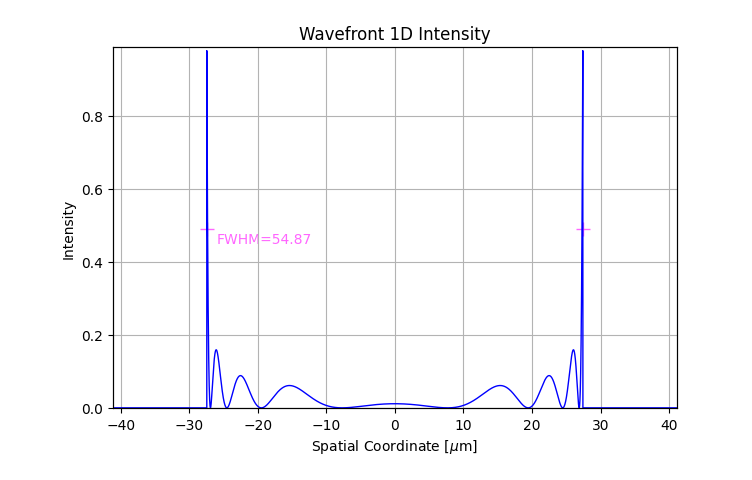
\includegraphics[width=1\textwidth]{figures/fig_Du_c111_17.png}
\end{figure}



In case of cylindrical bending, 
the displacement $\textbf{u(r)}$ can be expressed as a function of the elastic constants, and for the case if isotropic crystals [see \cite{Nesterets2008}] depends only on the coordinates, radius $R$, thickness $t$ and poisson ratio. The product $\textbf{h}\cdot\textbf{u}$ is given in equation (16) of \cite{GuigayFerrero2016}.

For a cylindrically \emph{bent} crystal, the field is given by equation (10) in \cite{GuigayFerrero2013} for the {\it symmetrical} Laue crystal: 

\begin{equation}\label{eq:Dx0symmetrical}
    D_h(x) =
J_{0}\!\left(
Z\sqrt{a^2-x^2}\right)\,
\exp\!\Bigl[-i k\,\frac{x(x+a)}{2 R \cos\theta_B}\Bigr].
\end{equation}


For the {\it asymmetrical} crystal, the expression is given in \cite{GuigayFerrero2016} [see just before equation (23)]: 

\begin{equation}\label{eq:prop_asymmetric}
D_h(x) =
M\!\left( i \beta, 1, i A \gamma \frac{a^2 - x^2}{\sin^2 2\theta_B}
\right)\,
\exp\!\Bigl[i k 
\Bigl(\omega x -
\frac{\mu_1 x^2 + x t_1 \sin\theta_1}{2 R}
\Bigr)\Bigr]
\end{equation}
where
$M$ is the Kummer function, were the arguments depend on
$A=-h \sin\alpha [1 + (\cos 2\alpha + \cos 2 \theta_B)(1+\rho_\nu)/2]/R$,
$\alpha$ is the asymmetry angle ($\alpha=0$ if symmetric),
$\rho_\nu$ is a term depending on the elasticity constants\footnote{For isotropic crystals discussed here, $\rho_\nu=\nu/(1-\nu)$, with $\nu$ the Poisson ratio.};
$\beta=\Omega/A$, 
$\Omega=(k^2/4) \chi_h \chi_{\bar{h}}$.

The phase term depends on
$\omega=\chi_0(1-\gamma)/(2 \sin 2 \theta_B)$, 
$\gamma=\cos \theta_1 / \cos \theta_2$,
$\theta_{1,2}=\alpha \pm \theta_B$, $t_1=t/\cos \theta_1$ and 
\begin{equation}
    \mu_{1,2}=\frac
{\sin\alpha (\sin^2\theta_{1,2} + \rho_\nu \cos^2\theta_{1,2})+\cos\alpha \sin 2\theta_{1,2}}
{\sin 2 \theta_B \cos \theta_B}. \nonumber
\end{equation}
As a sanity check, in the symmetric Laue $\alpha=0$, thus $1-\gamma=0$, in consequence $A=\omega=0$, and $\mu_{1,2}=1/\cos \theta_B$. This makes the phase of equation~(\ref{eq:prop_asymmetric}) equal to the phase of equation~(\ref{eq:prop_symmetric}). 
To see that the Kummer $M$ becomes Bessel $J_0$ is not so evident at a first look because $\beta \rightarrow \infty$. A careful look at the $G_h$ series [eq.~(9) in \cite{GuigayFerrero2016}] shows a recurrence term $a_n = \dfrac{\Omega + i A n}{n^2}\,a_{n-1}$, and for $A=0$ is $a_n = \dfrac{\Omega}{n^2}\,a_{n-1}$. These terms are at the definition of $M(i\beta, 1, iy)$ and $J_0\!\left(2\sqrt{\Omega\, s_o s_h}\right)$ respectively.
As a practical consequence, the code for calculating the symmetrical case must implement $J_0$ as in equation~(\ref{eq:prop_symmetric}), because the symmetric case cannot be obtained numerically by just input $\alpha=0$ in the equations of the asymmetric case~(\ref{eq:prop_asymmetric}).

%%%%%%%%%%%%%%%%%%%%%%%%%%%%%%%%%%%%%%%%%%%%%%%%%%%%
%
%%%%%%%%%%%%%%%%%%%%%%%%%%%%%%%%%%%%%%%%%%%%%%%%%%%%
\subsection{Field at the exit of a cylindrically bent crystal for any entrance field}\label{sec:anytopoint}

The previous expressions are obtained for a point source in the entrance crystal surface. It is easy to calculate $D_h(x)$ for any incident field $D_0(\tau)$ just by integration of $D_0(\tau)$ with the propagator going from a point with coordinate $\tau$ to another point with coordinate $x$ [equation (28) in \cite{GuigayFerrero2016}]
\begin{equation}\label{eq:anyD0}
    D_h(x) = \int_{\gamma (x-a)}^{\gamma (x+a)} D_0(\tau) P(x, \tau) d\tau
\end{equation}
The expression of $P(x,
\tau)$ is found just before equation (29) in \cite{GuigayFerrero2016}
\begin{equation}
    P(x, \tau) = M(i\beta, 1, i y') e^{i k S_P(x, \tau)}
\end{equation}
with $y'=A\gamma(a^2-(x-\tau/\gamma)^2)/\sin^2 2\theta_B$, and
% DELETED (incorrect): old S_P had nu merely renamed to tau, inconsistent with
% y' which uses nu = x - tau/gamma. Kept for trace; replaced by the equation below.
% \begin{equation}
%     S_P(x,\tau) = \tau \omega -
%     \frac{\mu_1 x^2 + x t_1 \sin\theta_1}{2 R} -
%     \frac{\gamma^2 \mu_2 (\tau-x)^2 - a_2 \gamma (\tau - x)}{2 R} +
%     \frac{g}{R}(a + x)(\tau - x),
% \end{equation}
\begin{equation}
    S_P(x,\tau) = \left(x - \frac{\tau}{\gamma}\right) \omega -
    \frac{\mu_1 x^2 + x t_1 \sin\theta_1}{2 R} -
    \frac{\mu_2 \tau^2 + a_2 \tau}{2 R} -
    \frac{g}{\gamma R}(a + x)\,\tau,
\end{equation}
where 
$t_1=t/\cos \theta_1$,
$a_2=(t/\cos\theta_B) (\cos\alpha \sin\theta_2 + \rho_\nu \sin\alpha \cos\theta_2)$, and
$g=A \gamma R / (k \sin^2 2\theta_B)$.

Fig.~\ref{fig:fig_Du_c111_17_slit} shows an example of calculation using equation~(\ref{eq:anyD0}). The input field $D_0(\tau)$ is considered constant (plane wave) and clipped by a slit of different apertures (from 100 to 10$^{-3}$ \SI{}{\micro\meter}), just before impinging a flat symmetric diamond 111 crystal. Observe the different diffracted patterns (at the crystal exit plane). Note that, as expected, the results when closing the slit approach the pattern in Fig.~\ref{fig:fig_Du_c111_17}.

\begin{figure}
\caption{Numerical evaluation of $|D_h(x)|^2$ at $E$=17 keV for a  symmetric \SI{155}{\micro\meter} thick flat Diamond 111 crystal ($R=\infty$) with a plane wave source limited at the crystal entrance surface by a slit of a) 100 um, b) 10 um, c) 1 um, d) 1 nm  calculated using equation~(\ref{eq:anyD0}).
}
\label{fig:fig_Du_c111_17_slit}
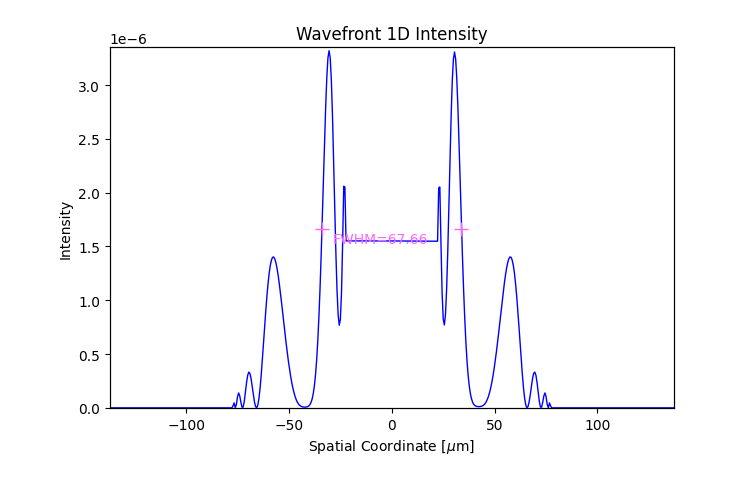
\includegraphics[width=0.48\textwidth]{figures/fig_Du_c111_17_slit_a.png}
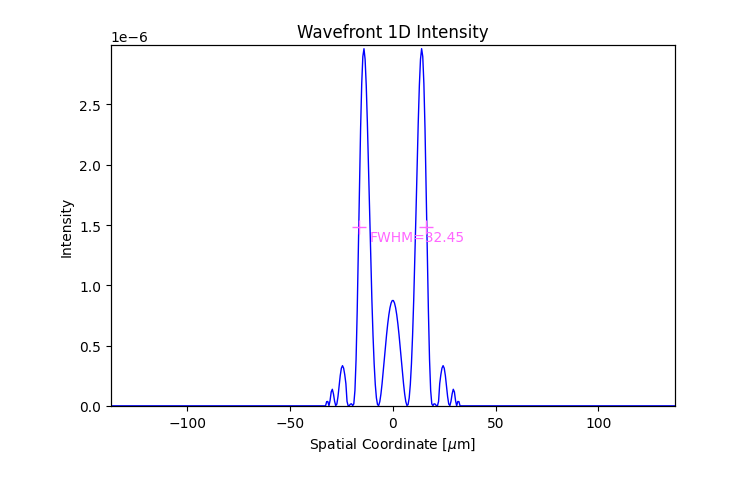
\includegraphics[width=0.48\textwidth]{figures/fig_Du_c111_17_slit_b.png}
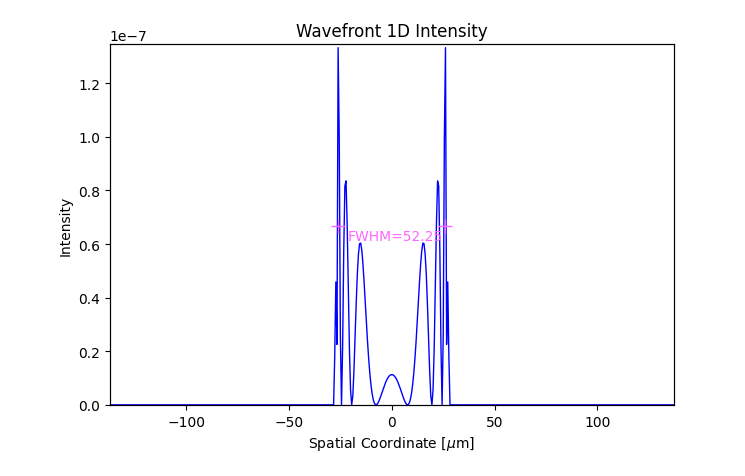
\includegraphics[width=0.48\textwidth]{figures/fig_Du_c111_17_slit_c.png}
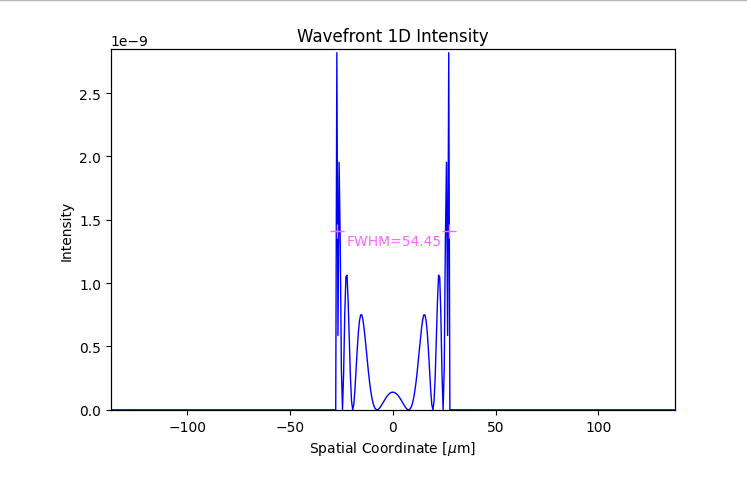
\includegraphics[width=0.48\textwidth]{figures/fig_Du_c111_17_slit_d.png}
\end{figure}


%%%%%%%%%%%%%%%%%%%%%%%%%%%%%%%%%%%%%%%%%%%%%%%%%%%%
%
%%%%%%%%%%%%%%%%%%%%%%%%%%%%%%%%%%%%%%%%%%%%%%%%%%%%
\subsection{Analytic expression for a \textit{cylindrically bent} Laue crystal when the source and observation points are distant from the crystal}
\label{sec:distantpandq}

In the particular case of a point source placed at a distance $p$ from the crystal,  we have,
\begin{equation}\label{eq:pointsource}
D_0(\tau)= \frac{e^{ik\frac{\tau^2}{2p}}}{\sqrt{i \lambda p}}.
\end{equation}
A compact expression of the diffracted field at the exit crystal is [equation (30) in \cite{GuigayFerrero2016}]
\begin{equation}\label{eq:anypandq0}
    D_h(x) = \int_{-a}^{a} 
    \frac{\gamma d\nu}{\sqrt{i \lambda p}}
    e^{i k \frac{\gamma^2 (x-\nu)^2}{2 p}}
    M(i\beta, 1, i y')
    e^{i k S_P(x, \nu)}
\end{equation}

Moreover, the diffracted field observed at any distance $q$ downstream from the exit surface can be calculated by propagation in vacuum of the field at the crystal exit ($q=0$). Using the Fresnel propagator
\begin{equation}\label{eq:fresnel}
    D_h(x,q) = \frac{e^{i k \frac{x^2}{2 q}}}{\sqrt{i \lambda q}} \int du~e^{i k \frac{(x-u)^2}{2q}} D_h(u)
\end{equation}

Compact expressions for a point source observed at $q$ are obtained in \cite{GuigayFerrero2016}. 
For point source on the crystal [$p=0$, ibid, equation (24)] 
\begin{equation}\label{eq:p0anaanyq}
    D_h(x,q) = 2
    \sqrt{
    \frac{e^{-k (t_1 + t_2 ) \chi_{0,\text{im}} / 2}}{\lambda \inred{|q|}}}
    \int_{0}^a du M(i\beta,1,i y')
    e^{i k \frac{u^2}{2 L_e}}
    \cos[k u (\frac{x-x_c}{q} - i ~ \omega_\text{im} ) ]
\end{equation}
with
$x_c = q(\omega_\text{re} - t_1 \sin\theta_1 / (2R))$ [ibid, equation (25)] the lateral shift of the pattern,
$\omega_\text{im}$ the imaginary part of $\omega$,\footnote{The term $\kappa = \chi_0 (t_1 - t_2)/ (4 a)$ used in our code is identical to $\omega = \chi_0 (1-\gamma)/(2 \sin 2\theta_B)$ as defined in \cite{GuigayFerrero2016} (using $a = t_1 \sin 2\theta_B / 2$ and $\gamma=t_2/t_1$), hence $\kappa_\text{im}=\omega_\text{im}$.} and
$L_e^{-1}=q^{-1} - \mu_1  R^{-1}$.

For a point source at finite distance $p$ [ibid, equation (31); derived in Appendix~\ref{app:singleintegral}]
% DELETED (inconsistent): the full-range integral and the cosine double-counted
% the folding, and the absorption belonged inside the cosine. Kept for trace;
% replaced by the folded form below (see Appendix~\ref{app:singleintegral}).
% \begin{equation}
%     D_h(x,q) =
%     e^{i k P_g}\, \gamma
%     \sqrt{
%     \frac{B_e\, e^{-k (t_1 + t_2 ) \chi_{0,\text{im}} / 2}}{\lambda q p}}
%     \int_{-a}^a du
%     M(i\beta,1,i y')
%     e^{i k u^2 / (2 L_e)}
%     e^{-k u \omega_\text{im}}
%     \cos[\frac{k u (x-x_c) B_e}{q p_e}],
% \end{equation}
\begin{equation}\label{eq:anypandanyq}
    D_h(x,q) = 2\,
    e^{i k P_g}\, \gamma
    \sqrt{
    \frac{B_e\, e^{-k (t_1 + t_2 ) \chi_{0,\text{im}} / 2}}{\lambda q p}}
    \int_{0}^a du
    M(i\beta,1,i y')
    e^{i k u^2 / (2 L_e)}
    \cos\left[k u \left(\frac{(x-x_c) B_e}{q p_e} - i\,\omega_\text{im}\right)\right],
\end{equation}
with
$P_g = \frac{x^2}{2 q} + \frac{(t_1+t_2) \chi_{0, \text{re}}}{4} - \frac{B_e}{2}\left(\frac{x}{q} + \frac{t_1 \sin\theta_1}{2 R} + m \right)^2$,
$B_e=(1/p_e + 1/q_e)^{-1}$,
$p_e= p R / (\gamma^2 (R - p \mu_2) - g p)$,
$q_e=q R / (R - q \mu_1 - g q)$,
$L_e^{-1} = (p_e+q_e)^{-1} + g/R$,
$x_c = q\left( \frac{p_e}{B_e}\omega_\text{re} + m\frac{p_e}{q_e} - \frac{t_1\sin\theta_1}{2R}\right)$ [ibid, equation (32)], and
$m=g a / R + \gamma (a_2 / (2R)) $.

Note that these expressions are also valid for the symmetric case ($\alpha=0, \gamma=1$) replacing $M(i\beta, 1, i y')$ by $J_0(Z \sqrt{a^2 - x^2})$.

These expressions are very useful for studying the focusing effect of a bent Laue crystal.
It has long been discussed that the dynamical effects do influence the focusing, and therefore the focus (position and size). It is inaccurate to use a simple geometrical lens equation that ignores dynamical effects [see \cite{guigaySanchezdelrio2022}].
The focal position can be calculated by plotting $|D(0,q)|^2$, as discussed in \cite{GuigayFerrero2013, GuigayFerrero2016}.
See an example in Fig.~\ref{fig_Dq_Si111_20_Dq}.


\begin{figure}
\caption{Calculations for a  symmetric \SI{250}{\micro\meter} thick flat Si 111 crystal ($R$=\SI{2}{m}) with source at the $p$=\SI{29}{m} upstream from the crystal at $E$=\SI{20}{keV}.
a) Numerical evaluation of $|D_h(0,q)|^2$ calculated using equation~(\ref{eq:anypandanyq}).
b) Numerical evaluation of $D_h(x,0)$ using equation~(\ref{eq:anypandq0}), and then propagated numerically to different $q$ distances to obtain (and display) the intensities $|D_h(x,q)|^2$.
}
\label{fig_Dq_Si111_20_Dq}
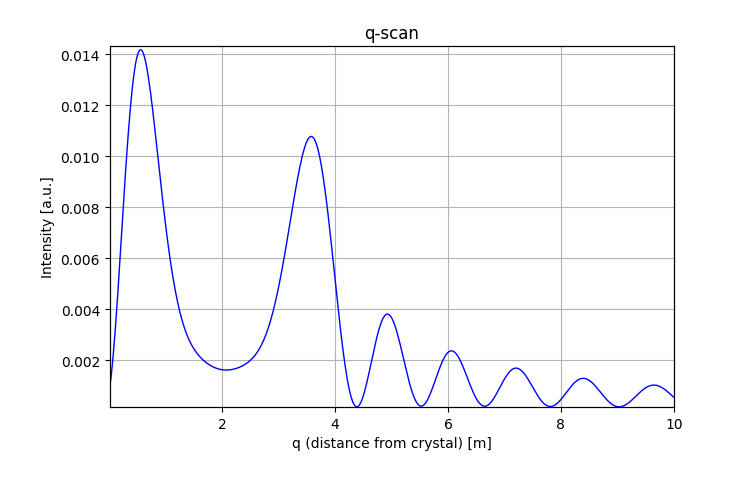
\includegraphics[width=1\textwidth]{figures/fig_Dq_Si111_20_Dq.png}
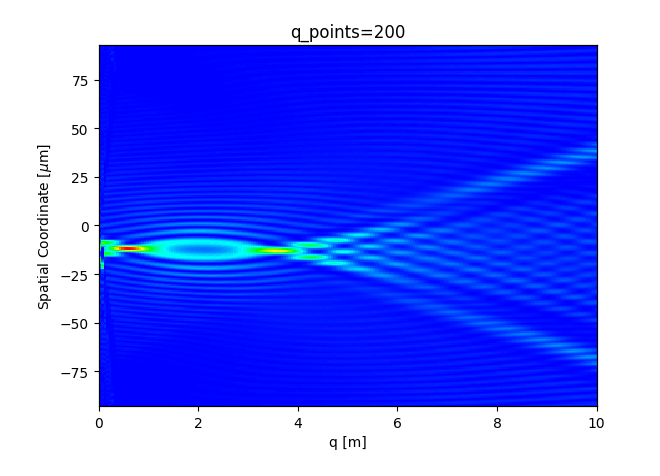
\includegraphics[width=1\textwidth]{figures/fig_Dq_Si111_20_map.png}
\end{figure}



%%%%%%%%%%%%%%%%%%%%%%%%%%%%%%%%%%%%%%%%%%%%%%%%%%%%
%
%%%%%%%%%%%%%%%%%%%%%%%%%%%%%%%%%%%%%%%%%%%%%%%%%%%%
\section{Examples of simulations}
\label{sec:results} 

%%%%%%%%%%%%%%%%%%%%%%%%%%%%%%%%%%%%%%%%%%%%%%%%%%%%
%
%%%%%%%%%%%%%%%%%%%%%%%%%%%%%%%%%%%%%%%%%%%%%%%%%%%%
\subsection{Benchmarking against published data}
\label{sec:banckmarking}
We first tested our code with the calculations shown in the figures of \cite{GuigayFerrero2016}. These examples use a Si111 crystal \SI{1}{\milli\meter} thick at \SI{80}{\kilo\eV} bent to $R=$\SI{2}{\meter} for different asymmetry angles and source position ($p=0$ for Fig. 2 and $p=$\SI{20}{\meter} in Fig. 3). Our results agree very well both in the $q$-scan (longitudinal) and the $x$-scan (transversal) at the focal position(s) (see Fig.~\ref{fig:GF2026figs23}). As a quantitative example, for the source at $p=$\SI{20}{\meter} and $\alpha=0.75^\circ$ (green curve in Fig.~\ref{fig:GF2026figs23}d) we obtain a focus at $q\approx$\SI{820}{\milli\meter} with a width FWHM$\approx$\SI{0.25}{\milli\meter}, in good agreement with the values of \SI{823.5}{\milli\meter} and \SI{0.23}{\milli\meter} reported in \cite{GuigayFerrero2016}.


\begin{figure}
\caption{Diffraction profiles at $E$=80 keV for \SI{1}{\milli\meter} thick Si111 bent ($R=$\SI{2}{\meter}) to reproduce the results in Figs. 2-3 of \cite{GuigayFerrero2016}: a) $q$-scan with the source at $p=$0; b)  $q$-scan with the source at $p=$\SI{20}{\meter}; c) transversal scans at focal positions for source at $p=$0; and d) transversal scans at focal positions for source at $p=$\SI{20}{\meter}.
}
\label{fig:GF2026figs23}
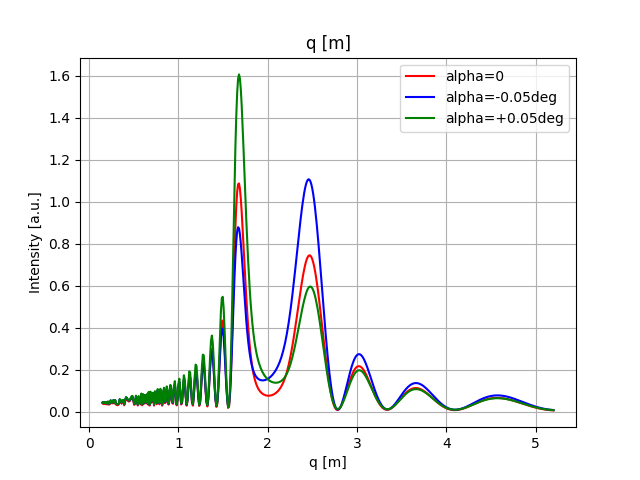
\includegraphics[width=0.45\textwidth]{figures/GF2016_fig2a.png}
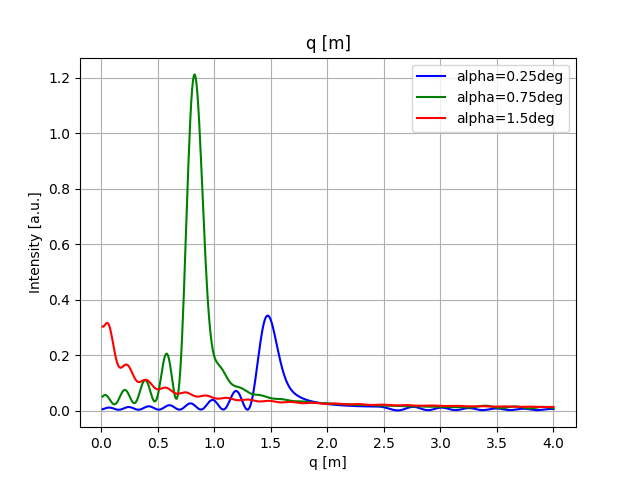
\includegraphics[width=0.45\textwidth]{figures/GF2016_fig3a.png}
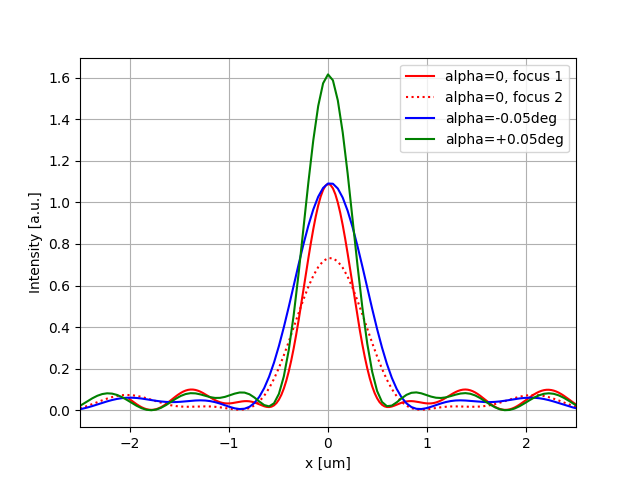
\includegraphics[width=0.45\textwidth]{figures/GF2016_fig2b.png}
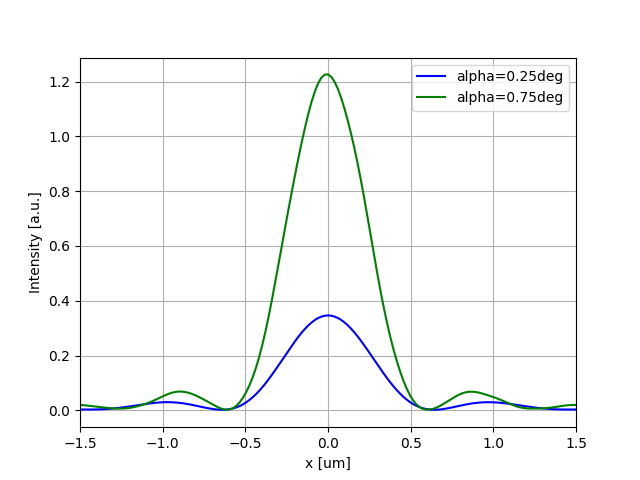
\includegraphics[width=0.45\textwidth]{figures/GF2016_fig3b.png}
\end{figure}


The Figs. 4-6 of \cite{GuigayFerrero2016} use a Si111 thin crystal (\SI{250}{\micro\meter}) at \SI{20}{\kilo\eV} bent also to $R=$\SI{2}{\meter}. The point source is placed at $p=$\SI{29}{\meter} for different asymmetry angles.
Looking to our results (see Fig.~\ref{fig:GF2026figs46}) we can make some remarks:
\begin{itemize}
    \item our curves for $\alpha > 0$ correspond to the curves for $\alpha < 0$ in \cite{GuigayFerrero2016}. We believe it was a mismatch of the labels in the plots in \cite{GuigayFerrero2016} (we used the same code as in calculations for Fig.~\ref{fig:GF2026figs23} that agreed well with the reference).
    \item Any residual difference in the relative heights of the two foci is small and is attributable to the slightly different magnitude of the susceptibilities used: our values, retrieved automatically with crystalpy \cite{guigaySanchezdelrio2024}, give $\chi_h\chi_{\bar h}=(1.67+0.017\,i)\times10^{-12}$ at \SI{20}{\kilo\eV}, about 1\% smaller in modulus than the XOP-tabulated value used in the references [$(1.68+0.017\,i)\times10^{-12}$, quoted in \cite{GuigayFerrero2013} for the same crystal]. The balance between the two foci is otherwise governed by the anomalous absorption discussed below, for which we adopt the same sign convention as the references.
    
\end{itemize}


\begin{figure}
\caption{Diffraction profiles at $E$=20 keV for \SI{250}{\micro\meter} thick Si111 bent ($R=$\SI{2}{\meter}) and point source at $p=$\SI{29}{\meter} to reproduce the results in Figs. 4-6 of \cite{GuigayFerrero2016}: a,b) $q$-scans (central intensity vs. $q$); c) transversal scans at the focal positions.
}
\label{fig:GF2026figs46}
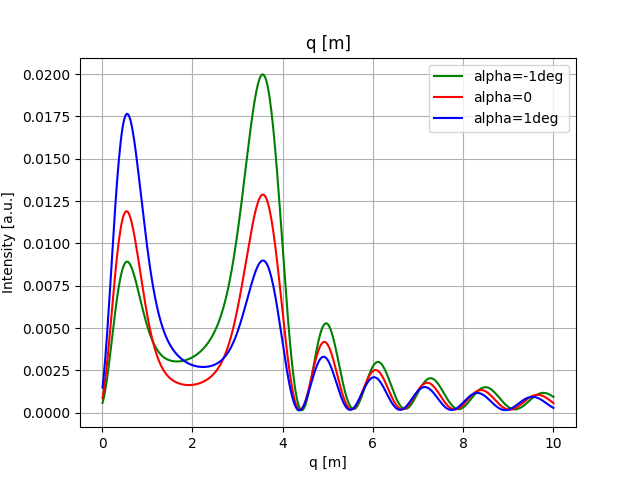
\includegraphics[width=0.32\textwidth]{figures/GF2016_fig4.png}
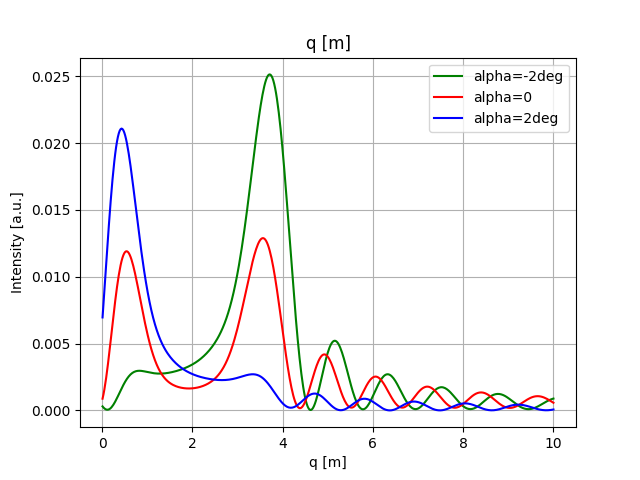
\includegraphics[width=0.32\textwidth]{figures/GF2016_fig5.png}
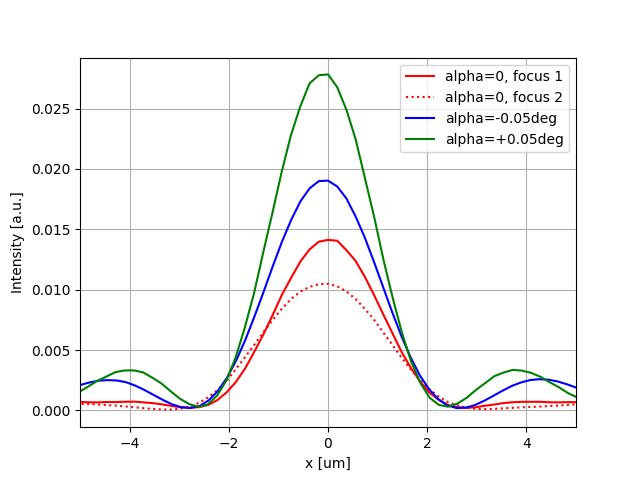
\includegraphics[width=0.32\textwidth]{figures/GF2016_fig6.png}
\end{figure}

Secondly, we benchmarked against the symmetric-Laue calculations of \cite{GuigayFerrero2013}. We reproduce their Figs.~4, 5 and~6 with good agreement, including the amplitudes: the \SI{20}{\kilo\eV} central-intensity ($q$-scan) curves and focal profiles for \SI{200}{} and \SI{300}{\micro\meter} thick Si~111 (Fig.~\ref{fig:GFBMP2013}), and the \SI{8.3}{\kilo\eV} curves for the same thicknesses (Fig.~\ref{fig:GFBMP2013fig6}).

A subtle point worth a comment concerns the imaginary part of the susceptibility product $\chi_h\chi_{\bar h}$, which controls the \emph{anomalous} (Borrmann) absorption. The reflected field can be written as the superposition of a convergent cylindrical wave, focusing at a real distance $q>0$, and a divergent one, with a virtual focus at $q<0$ \cite{GuigayFerrero2013}; the sign of $\text{Im}(\chi_h\chi_{\bar h})$ --- equivalently of $\text{Im}\,Z$, with $Z=\sqrt{\chi_h\chi_{\bar h}}\,k/\sin 2\theta_B$ --- selects which of the two is enhanced, and hence the shape of the intensity-versus-$q$ curve. This anomalous absorption is distinct from the \emph{normal} (photoelectric) absorption, which is governed by $\text{Im}\,\chi_0$ and gives the overall decaying factor $\exp[-k(t_1+t_2)\chi_{0,\text{im}}/2]$ in equations~(\ref{eq:p0anaanyq})--(\ref{eq:anypandanyq}).

We evaluate $\chi_h\chi_{\bar h}$ directly as the product $\chi_h\chi_{-h}$ of the $h$ and $-h$ Fourier components obtained from the structure factors [with crystalpy, \cite{guigaySanchezdelrio2024}]. For Si this gives $\text{Im}(\chi_h\chi_{\bar h})>0$, e.g. $\chi_h\chi_{\bar h}=(58.06+3.42\,i)\times10^{-12}$ at \SI{8.3}{\kilo\eV} and $(1.67+0.017\,i)\times10^{-12}$ at \SI{20}{\kilo\eV}, in agreement with the values quoted by \cite{GuigayFerrero2013} [$(57.81+3.26\,i)\times10^{-12}$ and $(1.68+0.017\,i)\times10^{-12}$, respectively; the residual $\sim1\%$ difference in modulus reflects the different tabulation of the atomic scattering factors]. With this choice all the figures of \cite{GuigayFerrero2013, GuigayFerrero2016} are reproduced. We note, however, that the sign of $\text{Im}(\chi_h\chi_{\bar h})$ is ultimately a convention, tied to the choice of time/propagation sign: the opposite (complex-conjugate) choice --- adopted for instance in Table~1 of \cite{guigaySanchezdelrio2022} --- simply mirrors the focusing curve in $q$.

This sign is, in any case, only of consequence when the anomalous absorption is significant, its effect scaling as $\text{Im}\,Z\times(\text{path length})$. At \SI{20}{\kilo\eV} (Figs.~4--5 of \cite{GuigayFerrero2013}) and at \SI{80}{\kilo\eV} (Fig.~\ref{fig:GF2026figs23}) the two foci have nearly equal height and the sign is immaterial; it becomes decisive only at \SI{8.3}{\kilo\eV} (Fig.~\ref{fig:GFBMP2013fig6}), where the convergent and divergent components interfere strongly and produce the characteristic structure reported in \cite{GuigayFerrero2013}. In practice this matters mostly for low-energy, strongly-absorbing applications --- for example the dispersive-EXAFS Laue polychromators operated around or below \SI{10}{\kilo\eV} --- where both the predicted focal position and the relative weight of the two foci depend on the susceptibility convention; getting it right then requires a consistent sign choice for $\chi_0$ (which fixes the normal-absorption decay) and for $\chi_h\chi_{\bar h}$. At the higher energies typical of most hard-X-ray beamlines the two foci are nearly symmetric and the issue is immaterial.


\begin{figure}
\caption{Diffraction profiles at $E$=20 keV for Si111 ($R$ is a function of $q$), source at $p=$\SI{29.7}{\meter}, reproducing the results in Figs. 4 and 5 of \cite{GuigayFerrero2013}:
a) thickness
\SI{200}{\micro\meter}: $q$-scan;
b) thickness
\SI{200}{\micro\meter}: intensity profile at focus $q=$\SI{0.5}{\meter} and $q=$\SI{0.75}{\meter};
c) thickness
\SI{300}{\micro\meter}: $q$-scan;
and d) thickness
\SI{300}{\micro\meter}: intensity profile at focus $q=$\SI{0.82}{\meter} and $q=$\SI{1.125}{\meter}.
}
\label{fig:GFBMP2013}
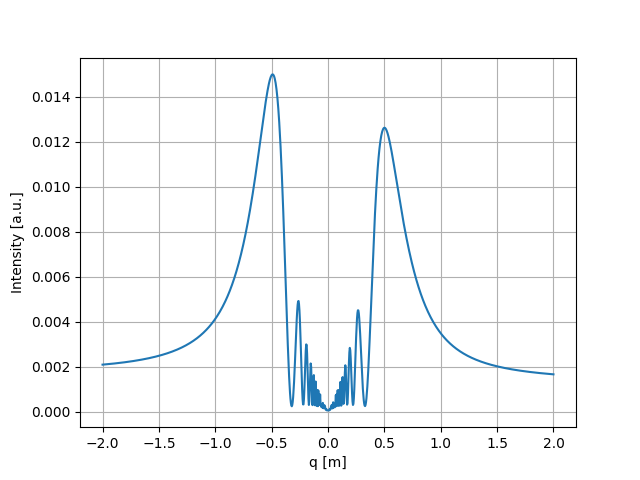
\includegraphics[width=0.45\textwidth]{figures/GFBMP2013_fig4a.png}
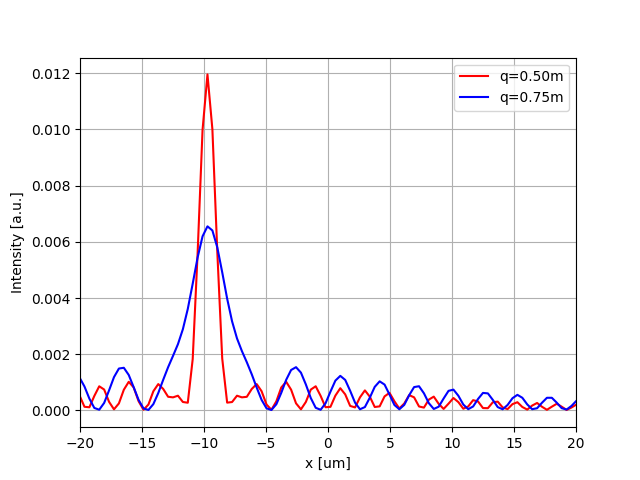
\includegraphics[width=0.45\textwidth]{figures/GFBMP2013_fig4b.png}
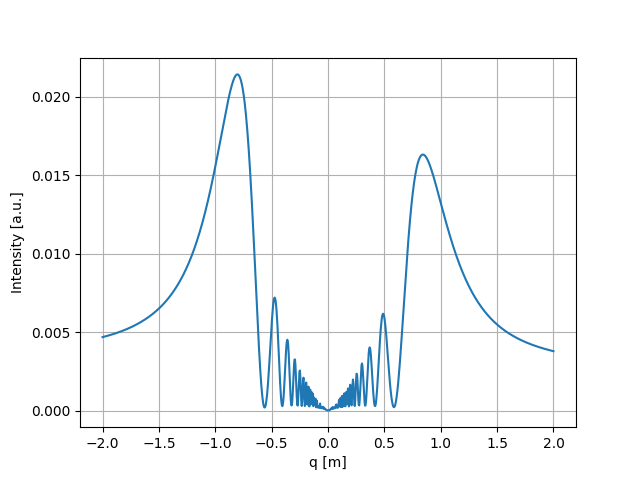
\includegraphics[width=0.45\textwidth]{figures/GFBMP2013_fig5a.png}
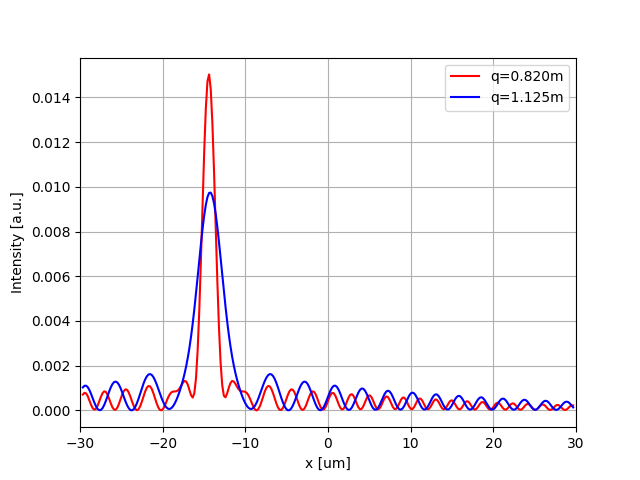
\includegraphics[width=0.45\textwidth]{figures/GFBMP2013_fig5b.png}
\end{figure}

\begin{figure}
\caption{Diffraction profiles at photon energy of \SI{8.3}{\kilo\eV} for Si111 ($R$ is a function of $q$), source at $p=$\SI{29.7}{\meter}, reproducing the results in Fig. 6 of \cite{GuigayFerrero2013}:
a) thickness
\SI{200}{\micro\meter}: $q$-scan;
b) thickness
\SI{300}{\micro\meter}: $q$-scan.
}
\label{fig:GFBMP2013fig6}
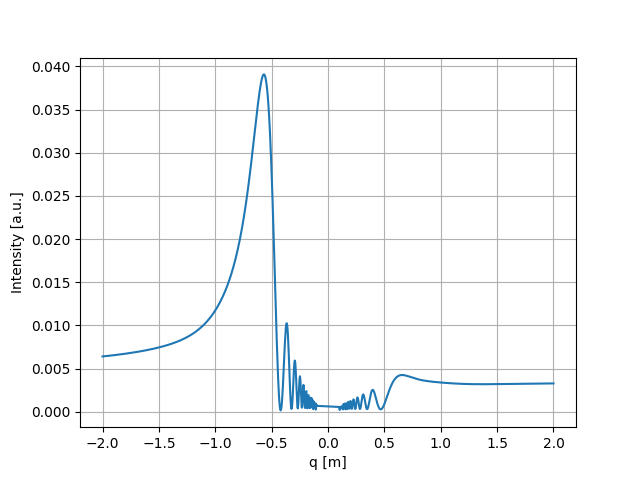
\includegraphics[width=0.45\textwidth]{figures/GFBMP2013_fig6a.png}
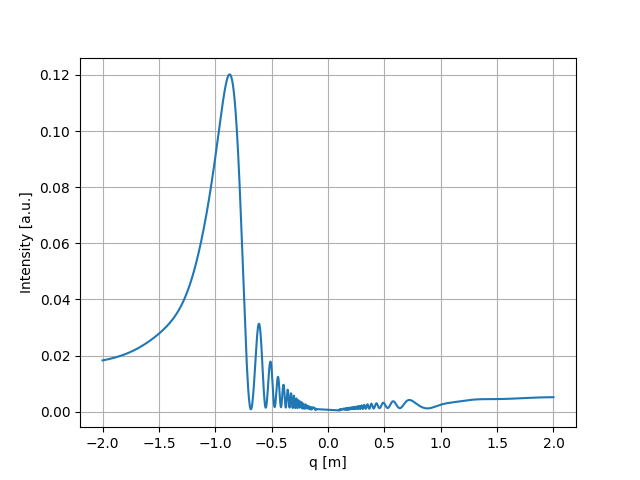
\includegraphics[width=0.45\textwidth]{figures/GFBMP2013_fig6b.png}
\end{figure}

Third, we re-calculate Figs. 4 and 5 from \cite{guigaySanchezdelrio2022}. The case of a symmetric Si111 Laue crystal of \SI{250}{\micro\meter} is analyzed at two photon energies (8.3 and \SI{17}{\kilo\eV}), for flat ($R=\infty$) or bent ($R=$\SI{1}{\meter}) cases and source at $p=0$ or $p=$\SI{50}{\meter}. Figure~\ref{fig:GSdR2022} shows the calculations with our code. The results differ from \cite{guigaySanchezdelrio2022} in a way that is entirely accounted for by the susceptibility convention discussed above: \cite{guigaySanchezdelrio2022} adopts the opposite (complex-conjugate) sign of $\chi_h\chi_{\bar h}$ --- its Table~1 lists $\text{Im}(\chi_h\chi_{\bar h})<0$, whereas we use $\text{Im}(\chi_h\chi_{\bar h})>0$, as in \cite{GuigayFerrero2013, GuigayFerrero2016}. For the flat crystal [Fig.~\ref{fig:GSdR2022}a,b] this mirrors the axial intensity profile in $q$: the strong (real) focus that \cite{guigaySanchezdelrio2022} place at $q>0$ appears here on the opposite side. For the bent crystal [Fig.~\ref{fig:GSdR2022}c,d], where both foci lie at $q>0$, the same sign change instead swaps the relative heights of the two foci (the dominant peak moves from the first focus to the second). Consistently with the absorption scaling discussed above, the effect is pronounced at \SI{8.3}{\kilo\eV} and weaker at \SI{17}{\kilo\eV}. The curves of \cite{guigaySanchezdelrio2022} are recovered exactly by taking the complex conjugate of $\chi_h\chi_{\bar h}$; we keep the structure-factor value here for consistency with the other benchmarks.


\begin{figure}
\caption{Diffraction profiles ($q$ scans) for Si111 discussing the results in Figs. 4 and 5 of \cite{guigaySanchezdelrio2022}:
a) source at $p=0$, $R=\infty$, photon energy \SI{8.3}{\kilo\eV};
b) source at $p=0$, $R=\infty$, photon energy \SI{17}{\kilo\eV};
c) source at $p=$\SI{50}{\meter}, $R=$\SI{1}{\meter}, photon energy \SI{8.3}{\kilo\eV};
d) source at $p=$\SI{50}{\meter}, $R=$\SI{1}{\meter}, photon energy \SI{17}{\kilo\eV}.
}
\label{fig:GSdR2022}
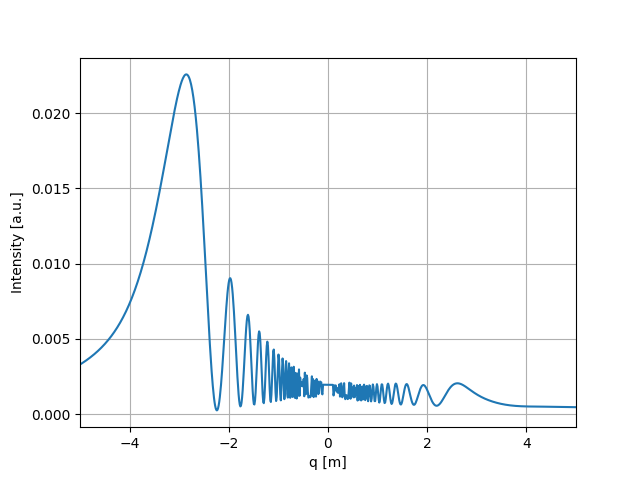
\includegraphics[width=0.45\textwidth]{figures/GSdR2022_fig4a.png}
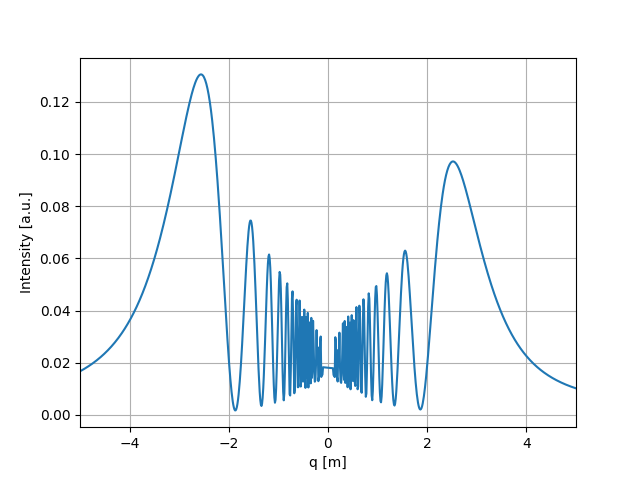
\includegraphics[width=0.45\textwidth]{figures/GSdR2022_fig4b.png}
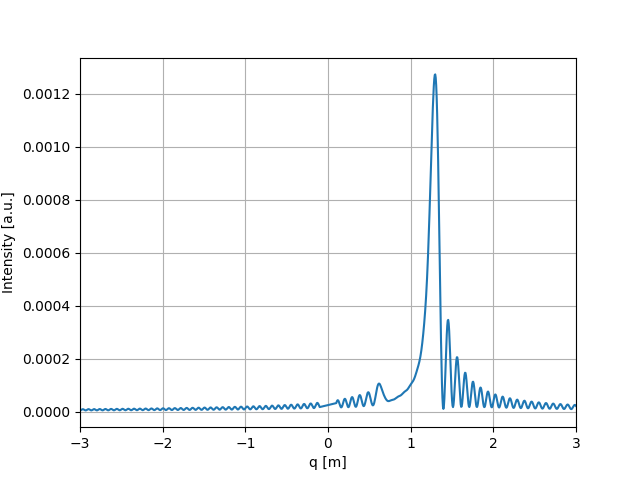
\includegraphics[width=0.45\textwidth]{figures/GSdR2022_fig5a.png}
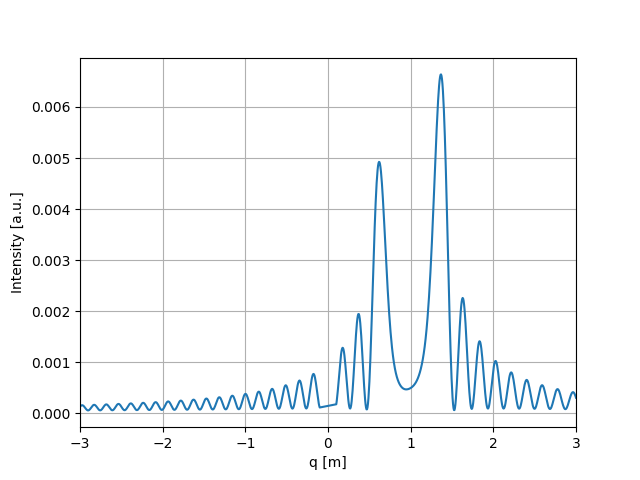
\includegraphics[width=0.45\textwidth]{figures/GSdR2022_fig5b.png}
\end{figure}


%%%%%%%%%%%%%%%%%%%%%%%%%%%%%%%%%%%%%%%%%%%%%%%%%%%%
%
%%%%%%%%%%%%%%%%%%%%%%%%%%%%%%%%%%%%%%%%%%%%%%%%%%%%
\subsection{Diffraction profiles}
\label{sec:diffractionprofiles}

In many cases, it is interesting to compute diffraction profiles. However, dealing with wave optics and curved crystals, it is not evident how to define, and therefore calculate them.

An incident plane wave is converted into another plane wave after diffraction (or transmission) by a flat crystal.
This permits to define easily the diffraction profiles (typically reflectivity vs. angle), because the directions (angles) of both incident and diffracted waves are well defined [see \cite{guigaySanchezdelrio2024}]. 

In wave optics, using the equations presented before, it is possible to calculate the diffracted field $D_h(x,q)$ at any position. 
Here, the angles or divergencies are related to far field observations.
Therefore, when propagating to a large distance $q_1$, where the Fraunhofer diffraction applies, the field $D_h$ can be expressed as a function of the angle $D_h(\theta)$, with $\theta=x / q_1$.
Where the Fraunhofer regime applies, the intensity distribution at two points $q_1$ and $q_2$ is the same when expressed as a function of the observation angle $\theta$. 

Considering that Fraunhofer propagator is the Fourier‑transform operator (with a constant amplitude factor and a quadratic‑phase term that we neglect for calculating intensities), we obtain the far‑field diffraction profile versus angle as the Fourier transform: 
\begin{equation}\label{eq:diffractionprofile1}
    |D(\theta)|^2 = \left| \int dx~e^{i k \theta x} D(x) \right|^2.
\end{equation}


We verified numerically that the diffraction profile of a flat crystal gives identical results when calculated by several methods [see Fig.~\ref{fig:diffractionprofile1}]:
\begin{enumerate}
    \item Compute the diffraction profile using the equations in \cite{guigaySanchezdelrio2024}
    [see Fig.~\ref{fig:diffractionprofile1}(a)]
    \item Perform the Fourier Transform [equation~(\ref{eq:diffractionprofile1})] of $D_h$ in equation~(\ref{eq:prop_symmetric})  [see Fig.~\ref{fig:diffractionprofile1}(b)]
    \item  
    Propagate numerically using the Fresnel propagator\footnote{the term in the exponent of equation~(\ref{eq:fresnel}) $\frac{(x-u)^2}{2q}$ becomes $\frac{-2xu}{2q}$ when $q \gg x,u$.}
    $D_h$ in equation~(\ref{eq:prop_symmetric}) to far field ($q_1$= 1 km)
    [see Fig.~\ref{fig:diffractionprofile1}(c)]
    \item  
    Obtain directly the propagated field at $q_1$= 1 km using equation~(\ref{eq:p0anaanyq})
    [see Fig.~\ref{fig:diffractionprofile1}(d)]
\end{enumerate}

\todo{How to ``normalize" the propagated ones, or the FT?}


\begin{figure}
\caption{Diffraction profiles at $E$=17 keV for a  symmetric \SI{155}{\micro\meter} thick flat Diamond 111 crystal computed by 4 different ways (see text). \todo{indicate the Bragg angle}
}
\label{fig:diffractionprofile1}
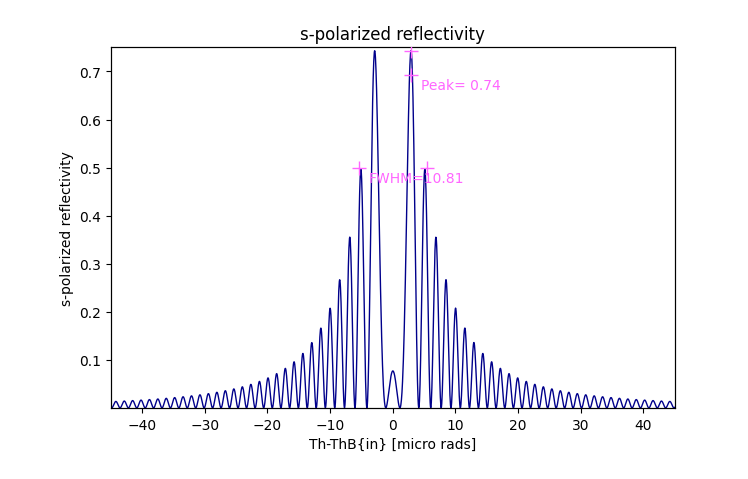
\includegraphics[width=0.45\textwidth]{figures/rc1.png}
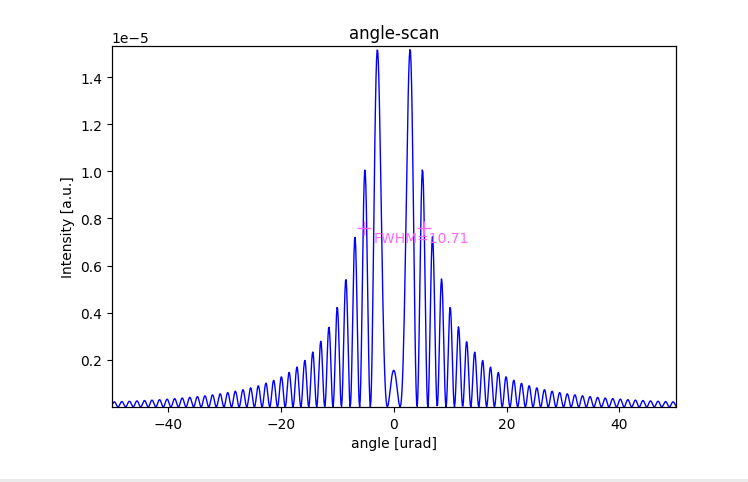
\includegraphics[width=0.45\textwidth]{figures/rc2.png}
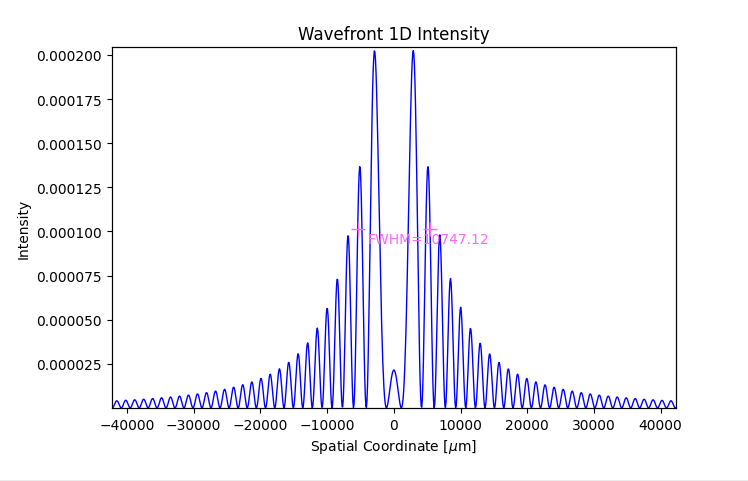
\includegraphics[width=0.45\textwidth]{figures/rc3.png}
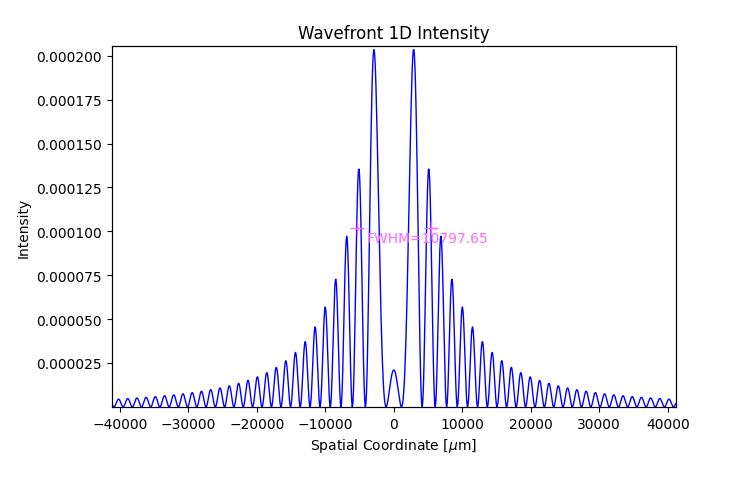
\includegraphics[width=0.45\textwidth]{figures/rc4.png}
\end{figure}



\begin{figure}
\caption{Diffraction profiles at $E$=17 keV for \SI{155}{\micro\meter} thick curved (R=1~m)  Diamond 111 crystal computed for $\alpha$=-10,0,10 degrees.
}
\label{fig:rcCurved}
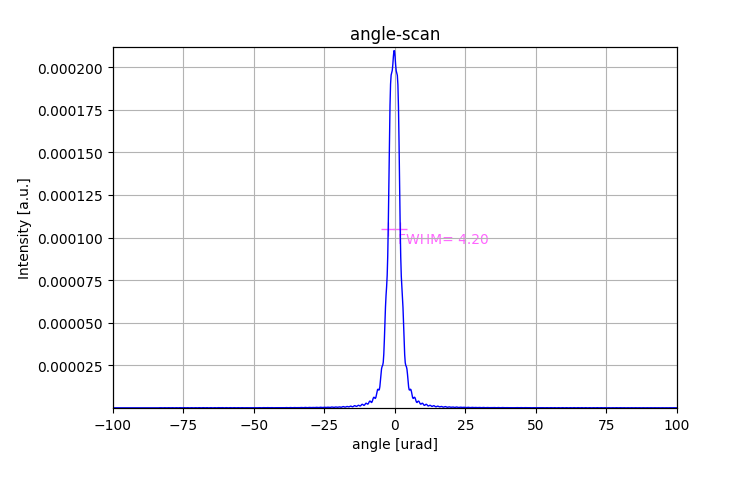
\includegraphics[width=0.7\textwidth]{figures/rc1m-10deg.png}
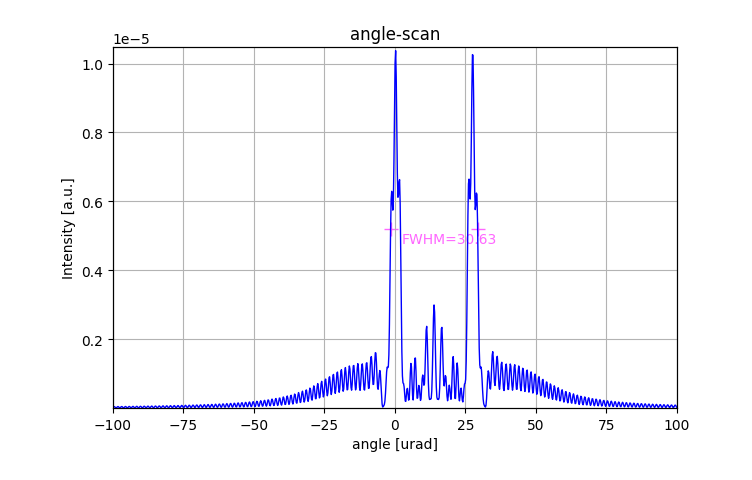
\includegraphics[width=0.7\textwidth]{figures/rc1m0deg.png}
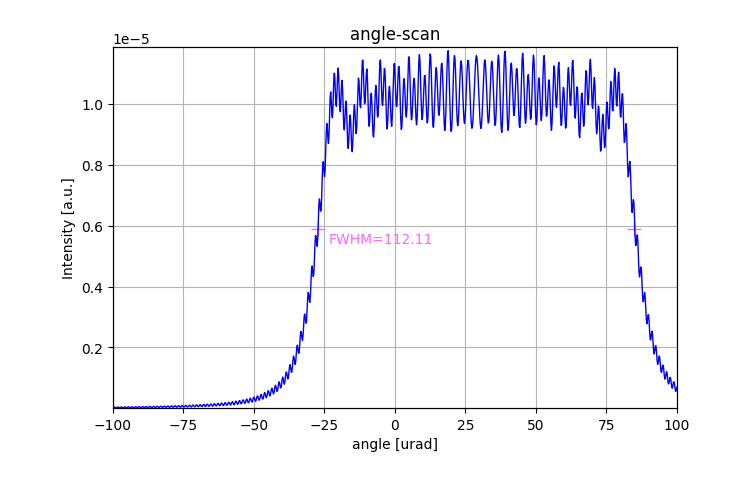
\includegraphics[width=0.7\textwidth]{figures/rc1m10deg.png}
\end{figure}

\begin{figure}
\caption{FWHM, peak and integrated intensity of the diffraction profiles vs asymmetry angle $E$=17 keV for \SI{155}{\micro\meter} thick curved (R=1~m)  $\theta_B$=10.2 deg; Diamond 111 crystal.
On the left column, this work, on the right, results using the Penning--Polder and Multilamellar methods described in \cite{codeCRYSTAL}
}
\label{fig:rcCurvedAlpha}
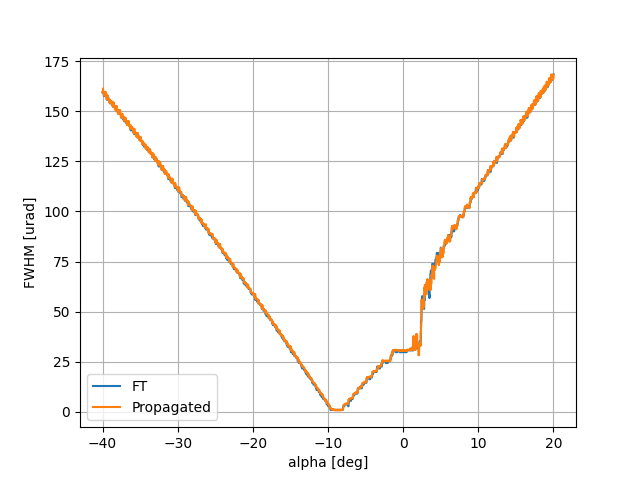
\includegraphics[width=0.49\textwidth]{figures/alpha_scan_fwhm.png}
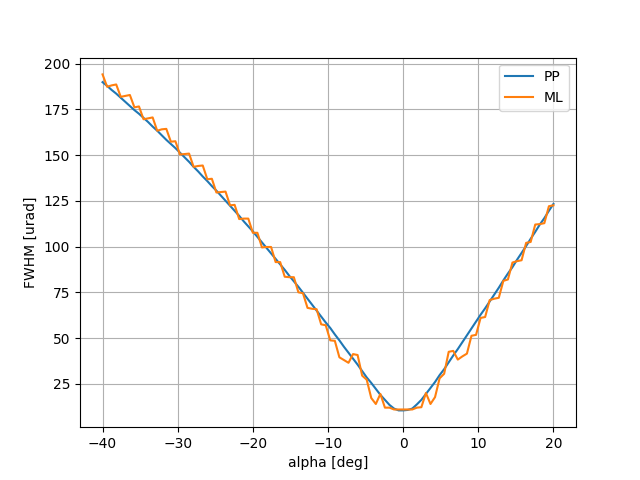
\includegraphics[width=0.49\textwidth]{figures/alpha_scan_fwhm_PPML.png}
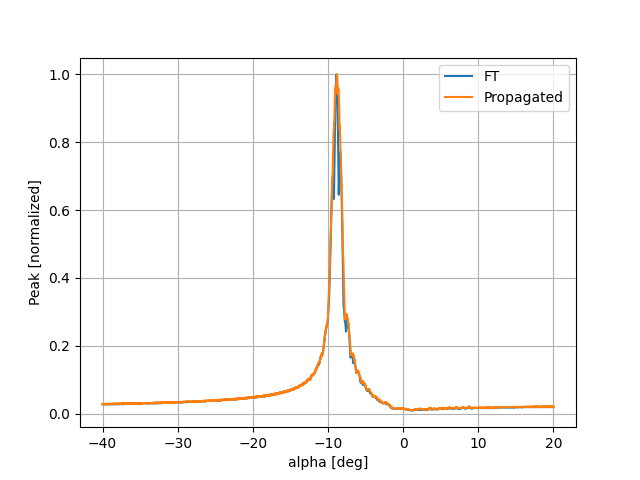
\includegraphics[width=0.49\textwidth]{figures/alpha_scan_peak.png}
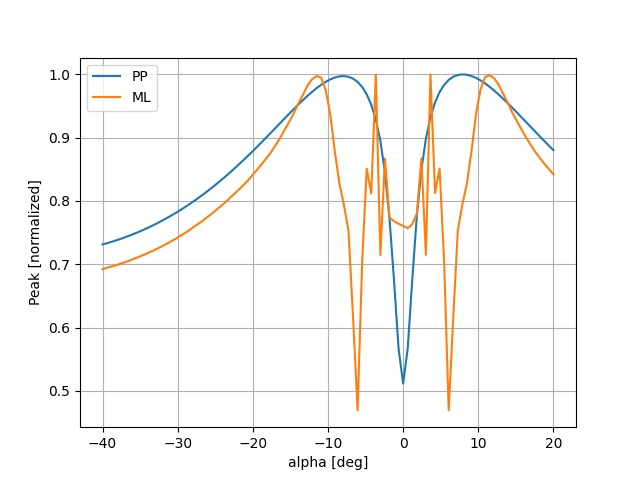
\includegraphics[width=0.49\textwidth]{figures/alpha_scan_peak_PPML.png}
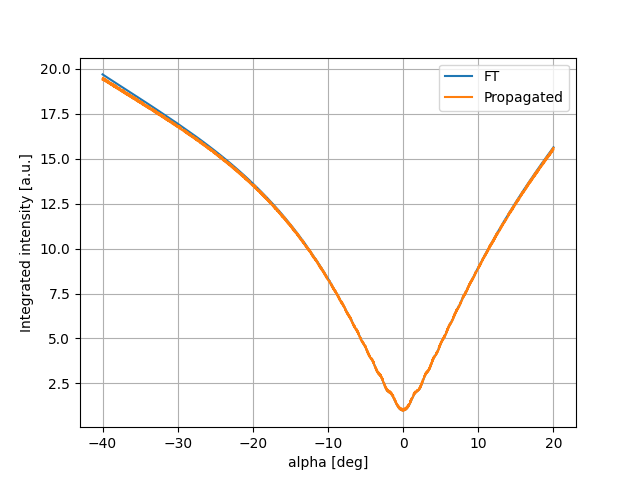
\includegraphics[width=0.49\textwidth]{figures/alpha_scan_integ.png}
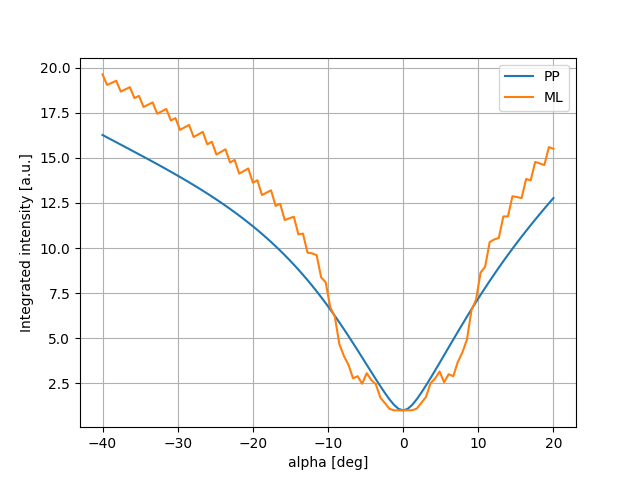
\includegraphics[width=0.49\textwidth]{figures/alpha_scan_integ_PPML.png}
\end{figure}

\begin{figure}
\caption{The same as in Figure~\ref{fig:rcCurvedAlpha} but for photon energy of 34500 eV and $\theta_B$=5 deg.
}
\label{fig:rcCurvedAlpha34}
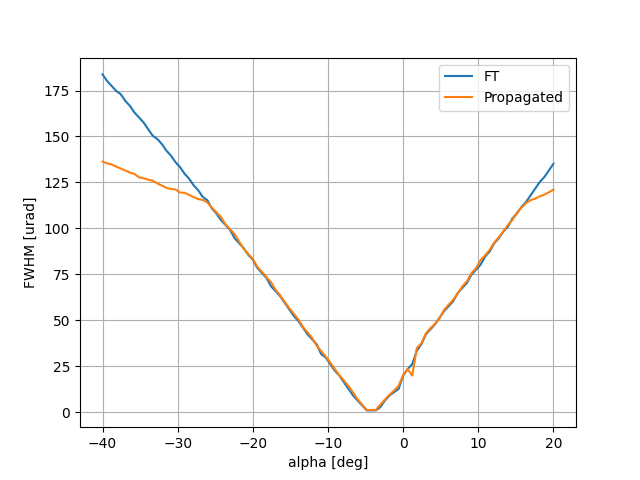
\includegraphics[width=0.49\textwidth]{figures/alpha_scan_fwhm34.png}
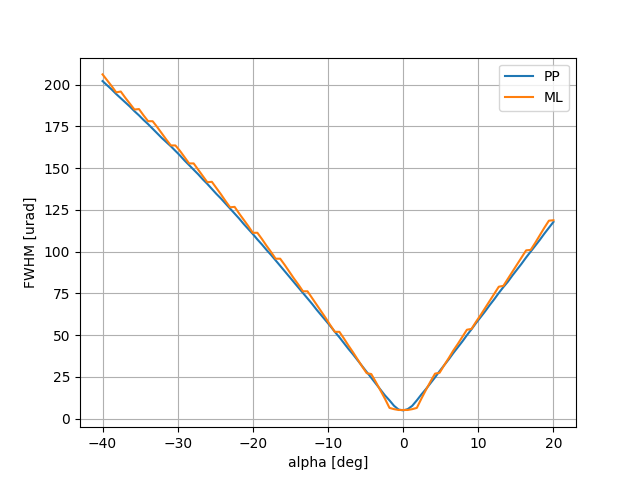
\includegraphics[width=0.49\textwidth]{figures/alpha_scan_fwhm34_PPML.png}
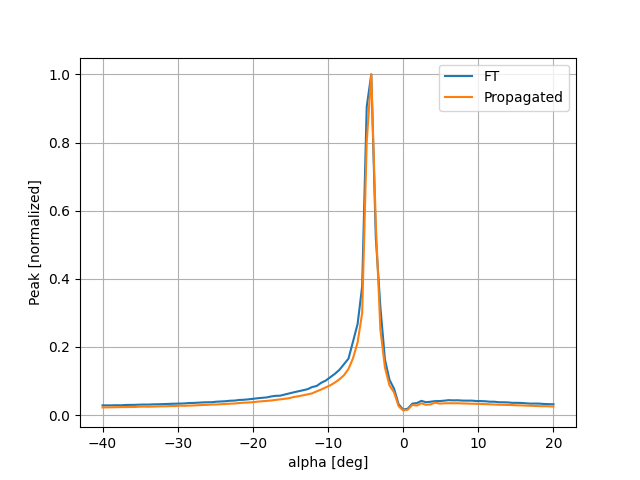
\includegraphics[width=0.49\textwidth]{figures/alpha_scan_peak34.png}
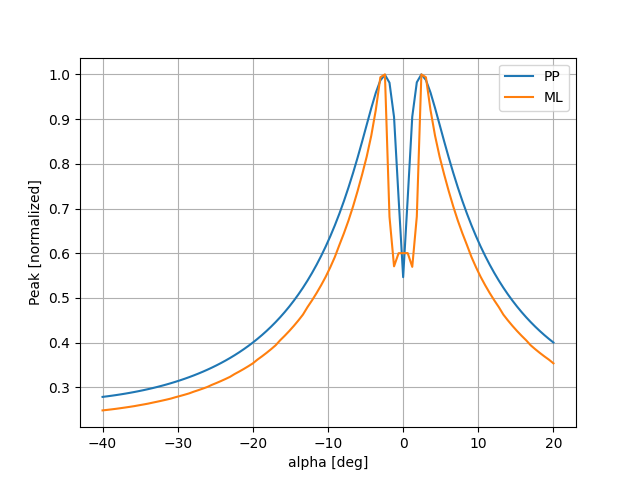
\includegraphics[width=0.49\textwidth]{figures/alpha_scan_peak34_PPML.png}
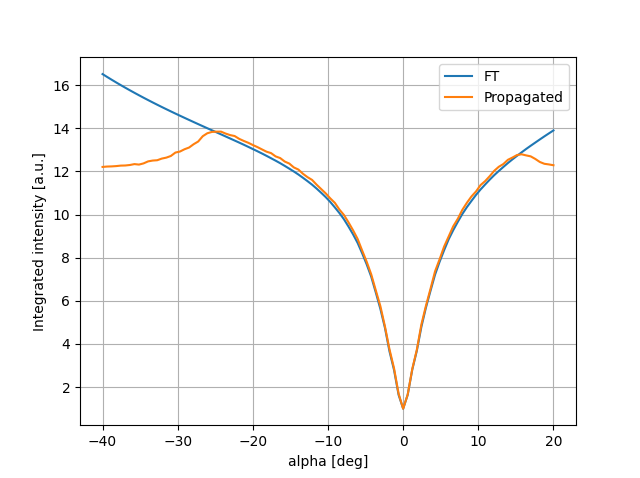
\includegraphics[width=0.49\textwidth]{figures/alpha_scan_integ34.png}
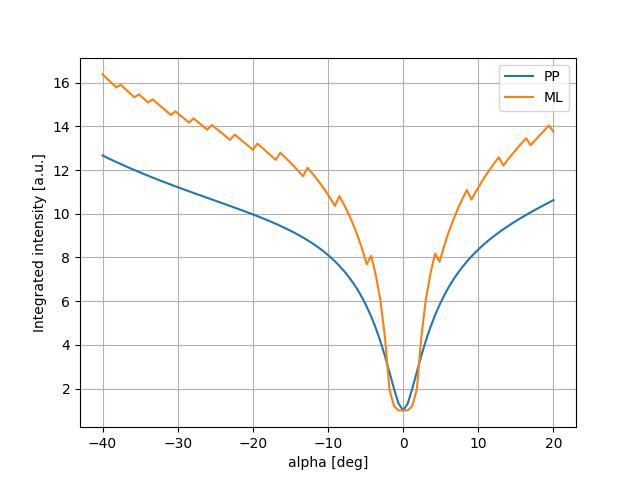
\includegraphics[width=0.49\textwidth]{figures/alpha_scan_integ34_PPML.png}
\end{figure}

Having checked the possibility to calculate the diffraction profile by propagation or by FT, we apply it to the curved crystal with $R$=\SI{1}{m}.
The results for $\alpha=-10,0,10$ degrees are shown in Fig.~\ref{fig:rcCurved}.

These calculations are useful for projecting a double-crystal Laue-Laue monochromator. Practically, the crystals are bent to increase the integrated reflectivity and therefore the outcoming flux. However, the curved crystals also produce an undesired dispersion energy-position at the diffraction beam. To minimize this, the crystal must be bent to fit the source in the Rowland, circle. Moreover, the resulting energy bandwidth $\Delta E/E$ is proportional to the diffraction width and must be fitted to experimental requirements, this making a compromise between flux and resolution. The parameters of the crystal that can be optimized are: asymmetry angle and crystal thickness. In Fig.~\ref{fig:id11} we display the $\alpha$ scan for the Si 111 Laue crystal to be used at the ESRF-ID11 monochromator. 


\begin{figure}
\caption{FWHM and integrated intensity of the diffraction profiles vs asymmetry angle $E$=40 keV for \SI{2500}{\micro\meter} thick curved Si 111 crystal. The scan has been performed for a fixed curvature ($R=$cte) and for a variable curvature matching the Rowland condition. Optimum values of reflectivity are obtained around $\alpha \approx 50$ degrees.
}
\label{fig:id11}
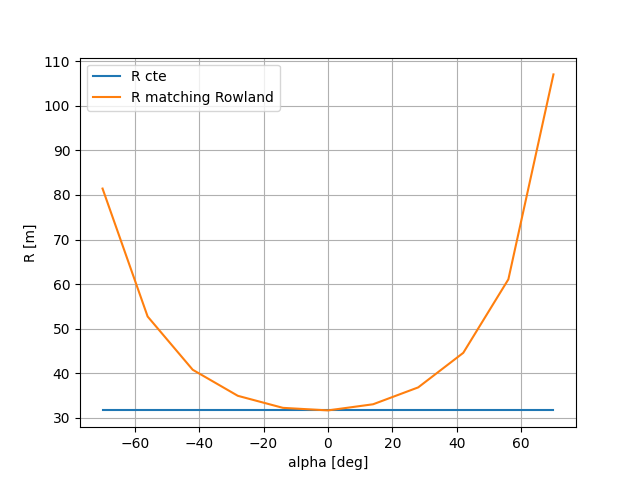
\includegraphics[width=0.6\textwidth]{figures/id11_R.png}
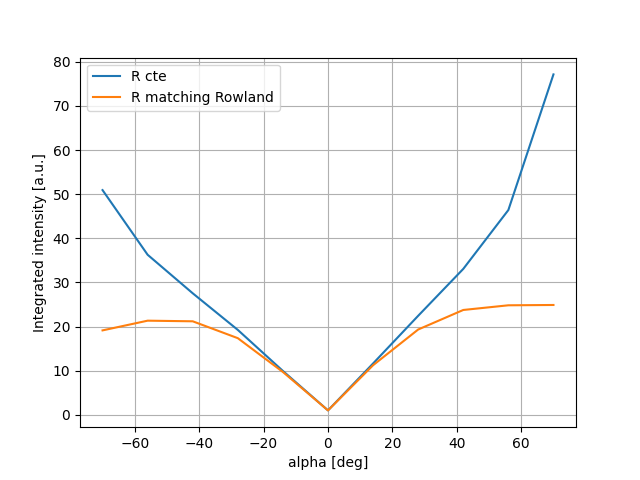
\includegraphics[width=0.6\textwidth]{figures/id11_I.png}
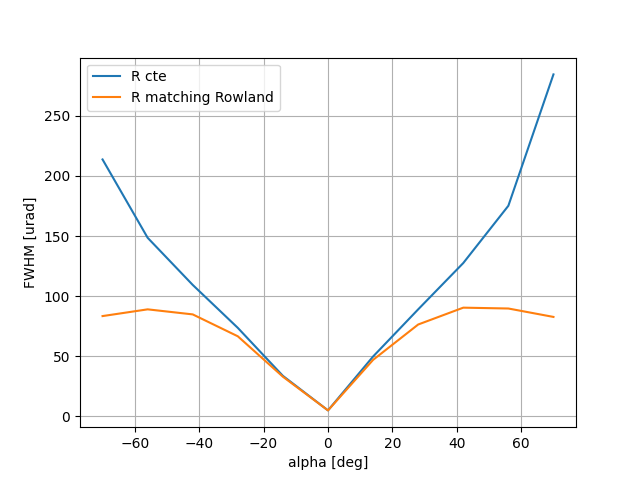
\includegraphics[width=0.6\textwidth]{figures/id11_FWHM.png}
\end{figure}


%%%%%%%%%%%%%%%%%%%%%%%%%%%%%%%%%%%%%%%%%%%%%%%%%%%%
%
%%%%%%%%%%%%%%%%%%%%%%%%%%%%%%%%%%%%%%%%%%%%%%%%%%%%
\section{Summary and conclusions}
\label{sec:summary}

We have presented the implementation of curved Laue crystals in the wavefront propagation framework WOFRY, part of the OASYS suite. The crystal is treated as a non-thin optical element: the diffracted field at the exit surface is obtained from the incident field by means of a crystal propagator (a point-spread or influence function) derived from the dynamical theory of diffraction, and it is then propagated in vacuum to any observation plane using the standard WOFRY free-space propagators. This scheme integrates naturally with the other WOFRY optical elements (sources, slits, lenses, mirrors), allowing the simulation of a curved Laue crystal as one component within a complete beamline.

The crystal propagator is based on the semi-analytical solution of the Takagi--Taupin equations developed by \cite{GuigayFerrero2013, GuigayFerrero2016}, valid for a constant strain gradient as produced by cylindrical bending. We have collected and used the relevant expressions: the Bessel-function influence function of the flat symmetric crystal \cite{kato1961, Guigay1999}, its generalization to the bent symmetric crystal \cite{GuigayFerrero2013}, and the confluent hypergeometric (Kummer) influence functions of the bent asymmetric crystal \cite{GuigayFerrero2016}, together with the compact single-integral forms for a point source and observer at arbitrary distances $p$ and $q$. The implementation covers both the symmetric ($\alpha=0$) and the general asymmetric geometry; as discussed in Section~\ref{sec:flat}, the symmetric case is computed directly with the Bessel-function form rather than as a numerical limit of the Kummer form.

We have benchmarked the implementation in several ways. The diffracted field of a flat crystal computed from the analytic influence function reproduces the expected behaviour both for a point source on the entrance surface and for a slit-limited plane wave, where the pattern tends to the point-source limit as the slit is closed (Figs.~\ref{fig:fig_Du_c111_17}, \ref{fig:fig_Du_c111_17_slit}). For bent crystals, the dynamical focusing is recovered by following the central intensity $|D_h(0,q)|^2$ as a function of distance, in agreement with the two-focus (symmetric) and single-focus (asymmetric) behaviour reported in \cite{GuigayFerrero2013, GuigayFerrero2016} (Fig.~\ref{fig_Dq_Si111_20_Dq}). We have also shown that diffraction profiles (reflectivity versus angle) can be obtained consistently from the far-field limit of the propagated field, either by Fourier transform or by numerical propagation, and that for a flat crystal the four independent methods give identical results (Fig.~\ref{fig:diffractionprofile1}). For curved crystals the computed profiles agree with those obtained with the Penning--Polder and multilamellar methods of \cite{codeCRYSTAL} (Figs.~\ref{fig:rcCurvedAlpha}, \ref{fig:rcCurvedAlpha34}).

Finally, we have illustrated the practical usefulness of these calculations for the design of double-crystal Laue--Laue monochromators, where the asymmetry angle, crystal thickness and bending radius can be optimized to trade off integrated reflectivity (flux) against energy bandwidth (resolution) while keeping the source on the Rowland circle. The scan of the diffraction properties versus asymmetry angle for the Si~111 crystal foreseen at the ESRF-ID11 monochromator (Fig.~\ref{fig:id11}) is an example of the kind of study this tool enables.

The present work is restricted to a 1D model and to monochromatic radiation. The dynamical focusing described here can be combined with polychromatic (geometric) focusing \cite{GuigayFerrero2013, PengQi, PengQi2021}; extending the implementation to polychromatic sources and to a full 2D treatment, as well as combining several crystals into complete monochromator and analyser systems, are natural directions for future work.


% \ack{Acknowledgements} 

\newpage

\bibliography{iucr} % reads iucr.bib with items
\bibliographystyle{iucr}


%#######################################
%#######################################

%#######################################
%#######################################
\appendix

\section{Displacement field of a cylindrically bent crystal}
\label{app:bent}

We use the coordinate system of \cite{Nesterets2008} [their Fig.~15 and Appendix~A; see also Fig.~1 in \cite{GuigayFerrero2016}]: the axis $x$ lies in the diffraction plane, parallel to the (unstrained) crystal surface, and the axis $z$ points into the crystal along the inward normal, with the origin at the mid-plane so that the entrance and exit faces are at $z=-t/2$ and $z=+t/2$, $t$ being the crystal thickness. The crystal is cylindrically bent with radius $R$ (taken positive for the geometry of \cite{Nesterets2008}, Fig.~15), the bending axis being perpendicular to the diffraction plane.

Assuming weak, isotropic deformations ($|x|,\,t \ll |R|$), the displacement field inside the crystal is [\cite{Nesterets2008}, equation~(16)]
\begin{align}
u_{x}(x,z) &= -\frac{xz}{R}, &
u_{z}(x,z) &= \frac{x^{2}+\rho_\nu\, z^{2}}{2R},
\qquad \rho_\nu=\frac{\nu}{1-\nu},
\end{align}
where $\nu$ is the Poisson ratio (the factor $\rho_\nu$ is denoted $K$ in \cite{Nesterets2008}).

The lattice deformation enters the Takagi--Taupin equations of Section~\ref{sec:TT} only through the phase $\mathbf{h}\cdot\mathbf{u}$, where $\mathbf{h}$ is the reciprocal-lattice vector of the reflection ($h=|\mathbf{h}|=2k\sin\theta_{B}$, $\theta_{B}$ being the Bragg angle). For an asymmetry angle $\alpha$ (angle between the diffraction planes and the crystal surface), the components of $\mathbf{h}$ in these axes are $h_{x}=-h\cos\alpha$ and $h_{z}=h\sin\alpha$ [\cite{GuigayFerrero2016}, equation~(15)], so that
\begin{equation}
\mathbf{h}\cdot\mathbf{u}
= \frac{h\cos\alpha}{R}\,xz
+ \frac{h\sin\alpha}{2R}\left(x^{2}+\rho_\nu\, z^{2}\right).
\end{equation}

In the symmetric Laue case ($\alpha=0$) this reduces to
\begin{equation}
\mathbf{h}\cdot\mathbf{u}
= \frac{h}{R}\,xz
= \frac{2k\sin\theta_{B}}{R}\,xz .
\end{equation}
This bilinear $xz$ term corresponds to a constant strain gradient; its integration along the Borrmann fan yields the curvature phase factor $\exp[-i k\,x(x+a)/(2R\cos\theta_{B})]$ of equation~(\ref{eq:Dx0symmetrical}) \cite{GuigayFerrero2013}, with $a=t\sin\theta_{B}$.

For the general asymmetric crystal the constant strain gradient is characterized by the parameter $A=-\partial^{2}(\mathbf{h}\cdot\mathbf{u})/\partial s_{o}\,\partial s_{h}$ \cite{authierbook}, with $s_{o}$ and $s_{h}$ the oblique coordinates along the incident and diffracted directions. Performing this change of variables [\cite{GuigayFerrero2016}, equations~(15)--(20)] gives
\begin{equation}
A=-\frac{h\sin\alpha}{R}
\left[1+\frac{1+\rho_\nu}{2}\left(\cos 2\alpha+\cos 2\theta_{B}\right)\right],
\end{equation}
which is the quantity entering the arguments of the Kummer functions in equations~(\ref{eq:prop_asymmetric})--(\ref{eq:anypandanyq}). Consistently, $A=0$ in the symmetric case, where the strain instead enters through the phase given above.


%%%%%%%%%%%%%%%%%%%%%%%%%%%%%%%%%%%%%%%%%%%%%%%%%%%%
\section{Derivation of the single-integral expressions for a distant point source}
\label{app:singleintegral}

This appendix derives the compact single-integral expressions~(\ref{eq:p0anaanyq}) and~(\ref{eq:anypandanyq}) for the Bragg-reflected field of a cylindrically bent Laue crystal, starting from the exit-surface field~(\ref{eq:anyD0}) and the vacuum propagator~(\ref{eq:fresnel}). The derivation follows \cite{GuigayFerrero2016} (their Section~5), adapted to the present notation.

\paragraph*{Setup.}
For a point source on the axis at a distance $p$ upstream of the crystal, the field on the entrance surface is $D_0(\tau)$ given by equation~(\ref{eq:pointsource}). Inserting the exit field~(\ref{eq:anyD0}) into the Fresnel integral~(\ref{eq:fresnel}) gives the field at an observation point $x$ located a distance $q$ downstream,
\begin{equation}\label{eq:appB_start}
D_h(x,q)=\frac{e^{ikx^2/(2q)}}{\sqrt{i\lambda q}}\int_{-\infty}^{\infty}\!\!du\;e^{ik\frac{(x-u)^2}{2q}}\int_{\gamma(u-a)}^{\gamma(u+a)}\frac{e^{ik\tau^2/(2p)}}{\sqrt{i\lambda p}}\,P(u,\tau)\,d\tau,
\end{equation}
where $u$ is the coordinate on the exit surface and the inner integral is the exit field~(\ref{eq:anyD0}).

\paragraph*{Change of variable.}
As in Section~\ref{sec:anytopoint}, set $\nu=u-\tau/\gamma\in[-a,a]$, so that $d\tau=\gamma\,d\nu$ and $P(u,\tau)=M(i\beta,1,iy')\,e^{ikS_P(u,\nu)}$ with $y'=A\gamma(a^2-\nu^2)/\sin^2 2\theta_B$ and [\cite{GuigayFerrero2016}, equation~(29)]
\begin{equation}
S_P(u,\nu)=\frac{(t_1+t_2)\chi_0}{4}+\nu\omega-\frac{\mu_1 u^2+ut_1\sin\theta_1}{2R}-\frac{\gamma^2\mu_2(\nu-u)^2-a_2\gamma(\nu-u)}{2R}+\frac{g}{R}(a+u)(\nu-u).
\end{equation}

\paragraph*{Total phase.}
Collecting the three quadratic phases in~(\ref{eq:appB_start}) (from the propagator, the source, and $S_P$) and setting aside the $u,\nu$-independent factors $e^{ikx^2/2q}$, $e^{iks^2/2p}$ (here the source is on axis, $s=0$) and $e^{ik(t_1+t_2)\chi_0/4}$ --- all restored below --- the integrand phase is $e^{ikS(u,\nu)}$ with
\begin{equation}
S(u,\nu)=\frac{u^2-2xu}{2q}+\frac{(\nu-u)^2}{2}\!\left(\frac{\gamma^2}{p}-\frac{\gamma^2\mu_2}{R}\right)+(\nu-u)\!\left(\frac{gu}{R}+m\right)-\frac{\mu_1u^2+ut_1\sin\theta_1}{2R}+\nu\omega,
\end{equation}
where $m=\dfrac{g a}{R}+\gamma\dfrac{a_2}{2R}$ (for $s=0$).

\paragraph*{Separation of $u$ and $\nu$.}
Grouping powers of $u$,
\begin{equation}
S(u,\nu)=\frac{B}{2}\,u^2-Cu+\frac{\nu^2}{2}\!\left(\frac{\gamma^2}{p}-\frac{\gamma^2\mu_2}{R}\right)+\nu(\omega+m),
\end{equation}
with
\begin{equation}
B=\frac{1}{p_e}+\frac{1}{q_e}=\frac{1}{B_e},\qquad
\frac{1}{p_e}=\frac{\gamma^2}{p}-\frac{\gamma^2\mu_2+g}{R},\qquad
\frac{1}{q_e}=\frac{1}{q}-\frac{\mu_1+g}{R},
\end{equation}
\begin{equation}
C=\frac{x}{q}+\frac{\nu}{p_e}+m+\frac{t_1\sin\theta_1}{2R}\equiv C_0+\frac{\nu}{p_e},\qquad
C_0=\frac{x}{q}+m+\frac{t_1\sin\theta_1}{2R}.
\end{equation}
The definitions of $p_e$ and $q_e$ invert to the forms quoted after equation~(\ref{eq:anypandanyq}).

\paragraph*{Integration over $u$.}
The Gaussian integral
\begin{equation}
\int_{-\infty}^{\infty}e^{ik(Bu^2/2-Cu)}\,du=\sqrt{i\lambda B_e}\;e^{-ikC^2/(2B)}
\end{equation}
is a function of $\nu$ through $C=C_0+\nu/p_e$. Writing $C^2=C_0^2+2C_0\nu/p_e+\nu^2/p_e^2$, the $\nu$-independent part $C_0^2$ adds a constant phase (collected into $P_g$ below), while the $\nu$- and $\nu^2$-terms combine with those already present in $S$.

\paragraph*{Focusing length and lateral shift.}
The resulting $\nu^2$ coefficient defines $L_e$,
\begin{equation}
\frac{1}{L_e}=\left(\frac{\gamma^2}{p}-\frac{\gamma^2\mu_2}{R}\right)-\frac{1}{Bp_e^2}=\frac{1}{p_e+q_e}+\frac{g}{R},
\end{equation}
where the second equality uses $Bp_e-1=p_e/q_e$. The $\nu$ coefficient is $\omega+m-C_0/(Bp_e)$; its imaginary part (carried entirely by $\omega$) produces the absorption factor $e^{-k\nu\omega_\text{im}}$, while equating its real part to $-(x-x_c)/(Bp_eq)$ yields [\cite{GuigayFerrero2016}, equation~(32)]
\begin{equation}
x_c=q\left(\frac{p_e}{B_e}\,\omega_\text{re}+\frac{p_e}{q_e}\,m-\frac{t_1\sin\theta_1}{2R}\right).
\end{equation}

\paragraph*{Restoring the prefactor.}
The real parts of the phases set aside above, together with the constant $-C_0^2/(2B)$ from the $u$-integration, combine into the global phase
\begin{equation}
P_g=\frac{x^2}{2q}+\frac{(t_1+t_2)\chi_{0,\text{re}}}{4}-\frac{B_e}{2}\left(\frac{x}{q}+\frac{t_1\sin\theta_1}{2R}+m\right)^2,
\end{equation}
while the imaginary part of $e^{ik(t_1+t_2)\chi_0/4}$ contributes the absorption amplitude $e^{-k(t_1+t_2)\chi_{0,\text{im}}/4}$. Multiplying the two square-root prefactors of~(\ref{eq:appB_start}) by $\sqrt{i\lambda B_e}$ from the $u$-integration gives $\gamma\sqrt{B_e/(i\lambda qp)}$ (the constant phase $\sqrt{1/i}$ is dropped).

\paragraph*{Folding.}
Since $y'$ and the $\nu^2$ phase are even in $\nu$ and the source is on axis, the interval $[-a,a]$ folds onto $[0,a]$, turning the $\nu$-linear factor $e^{-k\nu\omega_\text{im}}\,e^{-ik\nu(x-x_c)/(Bp_eq)}$ into a single cosine [using $\cosh(a+ib)=\cos(b-ia)$ and $1/(Bp_e)=B_e/p_e$]. Relabelling the integration variable $\nu\to u$, the result is
\begin{equation}\label{eq:appB_final}
D_h(x,q)=2\,e^{ikP_g}\,\gamma\sqrt{\frac{B_e\,e^{-k(t_1+t_2)\chi_{0,\text{im}}/2}}{\lambda qp}}
\int_0^a\!du\;M(i\beta,1,iy')\,e^{iku^2/(2L_e)}
\cos\!\left[ku\!\left(\frac{(x-x_c)B_e}{q\,p_e}-i\,\omega_\text{im}\right)\right],
\end{equation}
which is the compact form of equation~(\ref{eq:anypandanyq}). The special case of a source on the crystal ($p=0$) reduces~(\ref{eq:appB_final}) to equation~(\ref{eq:p0anaanyq}), with $1/q_e\to1/q-(\mu_1+g)/R$ and $L_e^{-1}\to q^{-1}-\mu_1R^{-1}$.


\end{document}                    % DO NOT DELETE THIS LINE
%%%%%%%%%%%%%%%%%%%%%%%%%%%%%%%%%%%%%%%%%%%%%%%%%%%%%%%%%%%%%%%%%%%%%%%%%%%%%%
